% !TEX root = ../main.tex/


\part{Answers to All Exercises}\newpage
%Solutions from Chapter 1

\section{Solutions to Exercises From Section 1}

\begin{solution}\label{sol:1.1}\ref{ex:1.1}
\begin{enumerate}
    \item $\{ 5x-1:x\in\Z \}=\{ \dots,-6,-1,4,9,\dots \}$.
    \item $\{ 3x+2:x\in\Z \}=\{ \dots,-1,2,5,8,\dots \}$. 
    \item $\{ x\in\Z: -2\le x\le 7\}=\{ -2,-1,0,1,2,3,4,5,6,7 \}$. 
    \item $\{ x\in\N:-2 < x \le 7 \}=\{ 0,1,2,3,4,5,6,7 \}$.
    \item $\{ x\in\R:x^2=3 \}=\{ -\sqrt 3, \sqrt 3 \}$.
    \item $\{ x\in\R:x^2=9 \}=\{ -3,3 \}$.
    \item $\{ x\in\R:x^2+5x=-6 \}=\{ -2,-3 \}$.
    \item $\{ x\in\R:x^3+5x^2=-6x \}=\{ -3,-2,0 \}$.
    \item $\{ x\in\R:\sin\pi x=0 \}=\Z$.
    \item $\{ x\in\R:\cos x=1 \}=\{ 2n\pi:n\in\Z \}$.
    \item $\{ x\in\Z:\lvert x \rvert<5 \}=\{ -4,-3,-2,-1,0,1,2,3,4 \}$.
    \item $\{ x\in\Z: \lvert 2x \rvert<5 \}=\{ -2,-1,0,1,2 \}$.
    \item $\{ x\in\Z:\lvert 6x \rvert<5 \}=\{ 0 \}$.
    \item $\{ 5x:x\in\Z,\lvert 2x \rvert\le8 \}=\{ -20,-15,-10,-5,0,5,10,15,20 \}$.
    \item $\{ 5a+2b:a,b\in\Z \}=\Z$.
    \item $\{ 6a+2b:a,b\in\Z \}=2\Z$.
\end{enumerate}

\end{solution}

\begin{solution}\label{sol:1.2}\ref{ex:1.2}
    \emph{Tip:} Some problems might look intimidating but in general, the easiest way to complete a problem like this, would be to consider the following three steps. 
    \begin{enumerate}
        \item [1] Is there common denominator? 
        \item [2] Is there a constant that can be factored out? 
        \item [3] What remains and how can this be generalised? 
    \end{enumerate}
    With those tips in mind, we proceed to the solutions. 
    \begin{enumerate}
        \item[17] $\{ 2,4,8,16,32,64 \}=\{ 2^x:x\in\N \}$
        \item[18] $\{ 0,4,16,36,64,100,\dots \}=\{ x^2:x\in\N,2\mid x \}$.
        \item[19] $\{ \dots,-6,-3,0,3,6,9,12,15,\dots \}=\{ 3x:x\in\Z \}$.
        \item[20] $\{ \dots,-8,-3,2,7,12,17,\dots \}=\{ 5x+2:x\in\Z \}$.
        \item[21] $\{ 0,1,4,9,16,25,36,\dots \}=\{ x^{2}:x\in\N\}$
        \item[22] $\{ 3,6,11,18,27,38,\dots \}=\{x^2+2:x\in\Z^{+}\}$
        \item[23] $\{ 3,4,5,6,7,8 \}=\{ x\in\N: 3\le x \le 8 \}$
        \item[24] $\{ -4,-3,-2,-1,0,1,2 \}=\{ x\in\Z:-4\le x \le 2 \}$
        \item[25] $\{ \dots,\frac{1}{8},\frac{1}{4},\frac{1}{2},1,2,4,8,\dots \}=\{x\in\Z: 2^{-x} \}$  
        \item[26] $\{ \dots,\frac{1}{27},\frac{1}{9},\frac{1}{3},1,3,9,27 \}=\{ 3^{-x}:x\in\Z \}$
        \item[27] $\{ \dots,-\pi,-\frac{\pi}{2},0,\frac{\pi}{2},\pi,\frac{3\pi}{2},2\pi,\frac{5\pi}{2} \}=\{ \frac{n\pi}{2}:n\in\Z \}$
        \item[28] $\{ \dots,-\frac{3}{2},-\frac{3}{4},0,\frac{3}{4},\frac{3}{2},\frac{9}{4},3,\frac{15}{4},\frac{9}{2},\dots \}=\{ \frac{3x}{4}:x\in\Z \}$   
    \end{enumerate}
\end{solution}

\begin{solution}\label{sol:1.3}\ref{ex:1.3}
    \begin{enumerate}
        \item[29] $\lvert \{ \{ 1 \},\{ 2,\{ 3,4 \} \},\varnothing \} \rvert=3$
        \item[30] $\lvert \{ \{ 1,4 \},a,b,\{ \{ 3,4 \} \},\{ \varnothing \} \} \rvert=5$
        \item[31] $\lvert \{ \{ \{ 1 \},\{ 2,\{ 3,4 \} \},\varnothing \} \} \rvert=1$
        \item[32] $\lvert \{ \{ \{ 1,4 \},a,b,\{ \{ 3,4 \} \},\{ \varnothing \} \} \} \rvert=1$  
        \item[33] $\lvert \{ x\in\Z:\lvert x \rvert<10 \} \rvert=19$
        \item[34] $\lvert \{x\in\N:\lvert x \rvert<10 \rvert\}=10$
        \item[35] $\lvert \{ x\in\Z:x^2<10 \} \rvert=7$
        \item[36] $\lvert \{ x\in\N:x^2<10 \} \rvert=4$
        \item[37] $\lvert \{ x\in\N:x^2<0 \} \rvert=0$
        \item[38] $\lvert \{ x\in\N:5x\le20 \} \rvert=5$.   
    \end{enumerate}
\end{solution}

\begin{solution}\label{sol:1.4}\ref{ex:1.4}
    \begin{enumerate}
        \item[39] $\{ (x,y):x\in[1,2],y\in[1,2] \}\Rightarrow$ This would be a solid $1\times 1$ square in $\R^2$ with corners $(1,1),(1,2),(2,1),(2,2)$
        \item[40] $\{ (x,y):x\in[0,1],y\in[1,2] \}\Rightarrow$ This would be a solid $1\times 1$ square in $\R^2$ with corners $(0,1),(0,2),(1,1),(1,2)$.
        \item[41] $\{ (x,y):x\in[-1,1],y=1 \}\Rightarrow$ This would be a line connecting $(-1,1)$ with $(1,1)$. 
        \item[42] $\{ (x,y):x=2,y\in[0,1] \}\Rightarrow$ This would be a line connecting $(2,0),(2,1)$    
        \item[43] $\{ (x,y):\lvert x \rvert=2,y\in[0,1] \}\Rightarrow$ This would be two vertical line segments, that connect $(-2,0)-(-2,1)$ and the other one would be $(2,0)-(2,1)$.
        \item[44] $\{ (x,x^2):x\in\R \}\Rightarrow$ This would be the parabolla $y=x^2$.
        \item[45] $\{ (x,y):x,y\in\R,x^2+y^2=1 \}\Rightarrow$ This would be the unit circle centered at the origin $(0,0)$ with $r=1$
        \item[46] $\{ (x,y):x,y\in\R,x^2+y^2\le 1 \}\Rightarrow$ This would be a disk with $r=1$, centered at $(0,0)$.
        \item[47] $\{ (x,y):x,y\in\R, y\ge x^2-1 \}\Rightarrow$ This would be the region underneath the parabola $y=x^2-1$.
        \item[48] $\{ (x,y):x,y\in\R x>1 \}\Rightarrow$ This would the whole upper right and down left quadrants of the $xy$-plane, or an \emph{open half-plane}, starting from $x=2$. 
        \item[49] $\{ (x,x+y):x\in\R,y\in\Z \}\Rightarrow$ This would be infinitely many parallel lines with slope $1$.
        \item[50] $\{ (x,\frac{x^2}{y})x\in\R,y\in\N\}\Rightarrow$ Division by $0$ is undefined, so we skip those values. Notice that the relation between the first and second coordinate is quadratic, instead of linear. That is to say $v=\frac{u^2}{k}$, so we have a upward-opening parabolas passing through the origin 
        \item[51] $\{ (x,y)\in\R^2:(y-x)(y+x)=0 \}\Rightarrow$ Here we have lines passing through the origin in an X shape. 
        \item[52] $\{ (x,y)\in\R^2:(y-x^2)(y+x^2)=0 \}\Rightarrow$ Lastly, we have two parabolas touching at the origin one opening upwards, one downwards, $y=x^2, y=-x^2$, respectively.
    \end{enumerate}
% --- FIRST PAGE: Items 39 to 45 ---
\begin{figure}[htbp]
    \centering
    \begin{subfigure}[b]{0.3\linewidth}
        \centering
        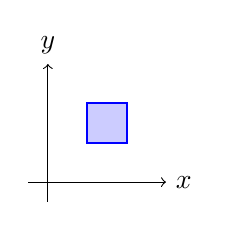
\begin{tikzpicture}[scale=0.5]
            \draw[->] (-0.5,0) -- (3,0) node[right] {$x$};
            \draw[->] (0,-0.5) -- (0,3) node[above] {$y$};
            \fill[blue!20] (1,1) rectangle (2,2);
            \draw[thick, blue] (1,1) rectangle (2,2);
        \end{tikzpicture}
        \caption{Item 39}
    \end{subfigure}\hfill
    \begin{subfigure}[b]{0.3\linewidth}
        \centering
        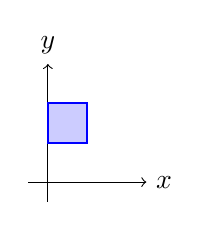
\begin{tikzpicture}[scale=0.5]
            \draw[->] (-0.5,0) -- (2.5,0) node[right] {$x$};
            \draw[->] (0,-0.5) -- (0,3) node[above] {$y$};
            \fill[blue!20] (0,1) rectangle (1,2);
            \draw[thick, blue] (0,1) rectangle (1,2);
        \end{tikzpicture}
        \caption{Item 40}
    \end{subfigure}\hfill
    \begin{subfigure}[b]{0.3\linewidth}
        \centering
        \begin{tikzpicture}[scale=0.5]
            \draw[->] (-2,0) -- (2,0) node[right] {$x$};
            \draw[->] (0,-0.5) -- (0,2) node[above] {$y$};
            \draw[very thick, blue] (-1,1) -- (1,1);
            \filldraw[blue] (-1,1) circle (2pt) (1,1) circle (2pt);
        \end{tikzpicture}
        \caption{Item 41}
    \end{subfigure}

    \vspace{0.5cm}

    \begin{subfigure}[b]{0.3\linewidth}
        \centering
        \begin{tikzpicture}[scale=0.5]
            \draw[->] (-0.5,0) -- (3,0) node[right] {$x$};
            \draw[->] (0,-0.5) -- (0,2) node[above] {$y$};
            \draw[very thick, blue] (2,0) -- (2,1);
            \filldraw[blue] (2,0) circle (2pt) (2,1) circle (2pt);
        \end{tikzpicture}
        \caption{Item 42}
    \end{subfigure}\hfill
    \begin{subfigure}[b]{0.3\linewidth}
        \centering
        \begin{tikzpicture}[scale=0.5]
            \draw[->] (-3,0) -- (3,0) node[right] {$x$};
            \draw[->] (0,-0.5) -- (0,2) node[above] {$y$};
            \draw[very thick, blue] (-2,0) -- (-2,1);
            \draw[very thick, blue] (2,0) -- (2,1);
            \filldraw[blue] (-2,0) circle (2pt) (-2,1) circle (2pt) (2,0) circle (2pt) (2,1) circle (2pt);
        \end{tikzpicture}
        \caption{Item 43}
    \end{subfigure}\hfill
    \begin{subfigure}[b]{0.3\linewidth}
        \centering
        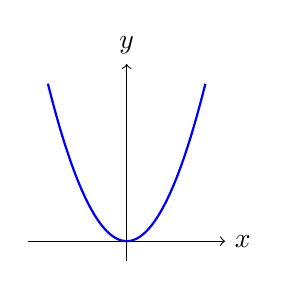
\begin{tikzpicture}[scale=0.5]
            \draw[->] (-2.5,0) -- (2.5,0) node[right] {$x$};
            \draw[->] (0,-0.5) -- (0,4.5) node[above] {$y$};
            \draw[thick, blue, domain=-2:2, samples=100] plot (\x, {\x*\x});
        \end{tikzpicture}
        \caption{Item 44}
    \end{subfigure}

    \vspace{0.5cm}

    \begin{subfigure}[b]{0.3\linewidth}
        \centering
        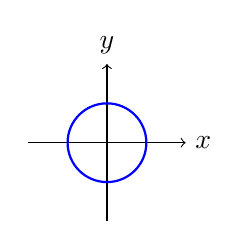
\begin{tikzpicture}[scale=0.5]
            \draw[->] (-2,0) -- (2,0) node[right] {$x$};
            \draw[->] (0,-2) -- (0,2) node[above] {$y$};
            \draw[thick, blue] (0,0) circle (1);
        \end{tikzpicture}
        \caption{Item 45}
    \end{subfigure}
    \caption{Geometric Representations 39--45}\label{fig:geom_part1}
\end{figure}
% --- SECOND PAGE: Items 46 to 52 ---
\begin{figure}[htbp]
    \ContinuedFloat% Keeps the figure numbering the same
    \centering
    \begin{subfigure}[b]{0.3\linewidth}
        \centering
        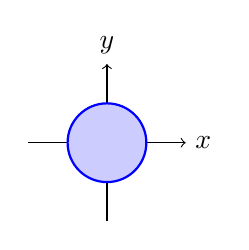
\begin{tikzpicture}[scale=0.5]
            \draw[->] (-2,0) -- (2,0) node[right] {$x$};
            \draw[->] (0,-2) -- (0,2) node[above] {$y$};
            \filldraw[fill=blue!20, draw=blue, thick] (0,0) circle (1);
        \end{tikzpicture}
        \caption{Item 46}
    \end{subfigure}\hfill
    \begin{subfigure}[b]{0.3\linewidth}
        \centering
        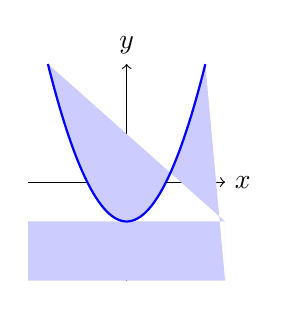
\begin{tikzpicture}[scale=0.5]
            \draw[->] (-2.5,0) -- (2.5,0) node[right] {$x$};
            \draw[->] (0,-2.5) -- (0,3) node[above] {$y$};
            \begin{scope}
                \clip (-2.5,-2.5) rectangle (2.5,3);
                \fill[blue!20] (-2.5,-2.5) rectangle (2.5,-1) -- plot[domain=-2:2, samples=100] (\x, {\x*\x - 1}) -- (2.5,-2.5);
                \draw[thick, blue, domain=-2:2, samples=100] plot (\x, {\x*\x - 1});
            \end{scope}
        \end{tikzpicture}
        \caption{Item 47}
    \end{subfigure}\hfill
    \begin{subfigure}[b]{0.3\linewidth}
        \centering
        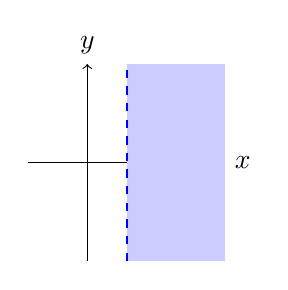
\begin{tikzpicture}[scale=0.5]
            \draw[->] (-1.5,0) -- (3.5,0) node[right] {$x$};
            \draw[->] (0,-2.5) -- (0,2.5) node[above] {$y$};
            \fill[blue!20] (1,-2.5) rectangle (3.5,2.5);
            \draw[dashed, thick, blue] (1,-2.5) -- (1,2.5);
        \end{tikzpicture}
        \caption{Item 48}
    \end{subfigure}

    \vspace{0.5cm}

    \begin{subfigure}[b]{0.3\linewidth}
        \centering
        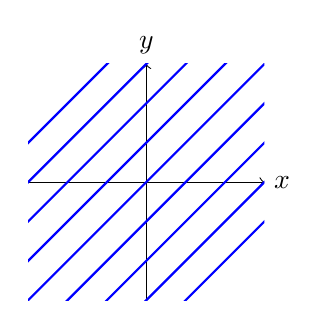
\begin{tikzpicture}[scale=0.5]
            \draw[->] (-3,0) -- (3,0) node[right] {$x$};
            \draw[->] (0,-3) -- (0,3) node[above] {$y$};
            \begin{scope}
                \clip (-3,-3) rectangle (3,3);
                \foreach \k in {-4,-3,...,4} {
                    \draw[thick, blue, domain=-4:4] plot (\x, {\x + \k});
                }
            \end{scope}
        \end{tikzpicture}
        \caption{Item 49}
    \end{subfigure}\hfill
    \begin{subfigure}[b]{0.3\linewidth}
        \centering
        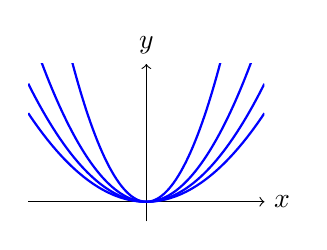
\begin{tikzpicture}[scale=0.5]
            \draw[->] (-3,0) -- (3,0) node[right] {$x$};
            \draw[->] (0,-0.5) -- (0,3.5) node[above] {$y$};
            \begin{scope}
                \clip (-3,-0.5) rectangle (3,3.5);
                \foreach \k in {1,2,3,4} {
                    \draw[thick, blue, domain=-3:3, samples=100] plot (\x, {(\x*\x)/\k});
                }
            \end{scope}
        \end{tikzpicture}
        \caption{Item 50}
    \end{subfigure}\hfill
    \begin{subfigure}[b]{0.3\linewidth}
        \centering
        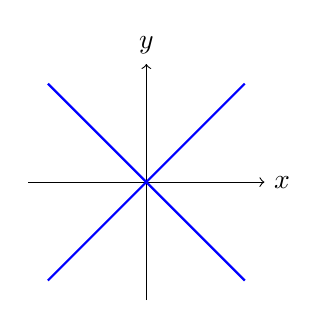
\begin{tikzpicture}[scale=0.5]
            \draw[->] (-3,0) -- (3,0) node[right] {$x$};
            \draw[->] (0,-3) -- (0,3) node[above] {$y$};
            \draw[thick, blue] (-2.5,-2.5) -- (2.5,2.5);
            \draw[thick, blue] (-2.5,2.5) -- (2.5,-2.5);
        \end{tikzpicture}
        \caption{Item 51}
    \end{subfigure}

    \vspace{0.5cm}

    \begin{subfigure}[b]{0.3\linewidth}
        \centering
        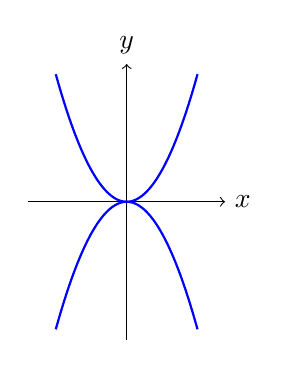
\begin{tikzpicture}[scale=0.5]
            \draw[->] (-2.5,0) -- (2.5,0) node[right] {$x$};
            \draw[->] (0,-3.5) -- (0,3.5) node[above] {$y$};
            \draw[thick, blue, domain=-1.8:1.8, samples=100] plot (\x, {\x*\x});
            \draw[thick, blue, domain=-1.8:1.8, samples=100] plot (\x, {-\x*\x});
        \end{tikzpicture}
        \caption{Item 52}
    \end{subfigure}

    \caption{Geometric Representations 46--52 (Continued)}\label{fig:geom_part2}
\end{figure}
\end{solution}

\section*{Solutions to Exercises from Section 2}
\begin{solution}\label{sol:2.1}\ref{ex:2.1}
$$
\begin{aligned}
    &(a) A\times B =\{ (1,a),(1,c),(2,a),(2,c),(3,a),(3,c),(4,a),(4,c) \}\\\\
    &(b) B\times A =\{ (a,1),(c,1),(a,2),(c,2),(a,3),(c,3),(a,4),(c,4) \}\\\\
    &(c) A\times A =A^2= \{ (1,1),(1,2),(1,3),(1,4),(2,1),(2,2),(2,3),\\\\
    &(2,4),(3,1),(3,2),(3,3),(3,4),(4,1),(4,2),(4,3),(4,4) \}\\
    &(d) B\times B = B^2 = \{ (a,a),(a,c), (c,a),(c,c) \}\\\\
    &(e) \varnothing\times B= \{ (a,b):a\in\varnothing,b\in B \}= \varnothing\\\\
    &(f) (A\times B)\times B = \{ (1,a),(1,c),(2,a),(2,c),(3,a),(3,c),(4,a),(4,c) \}\times
    \{ a,c \}=\\
    &\{ ((1,a),a),((1,c),a), ((2,a),a),\\
    &((2,c),a), ((3,a),a),((3,c),a),\\
    &((4,a),a),((4,c),a), ((1,a),c),\\ 
    &((1,c),c),((2,a),c),((2,c),c),\\
    &((3,a),c),((3,c),c),((4,a),c),((4,c),c) \}\\\\
    &(g) A\times (B\times B) = \{ 1,2,3,4 \}\times \{ (a,a),(a,c),(c,a),(c,c) \}=\\
    &\{ (1,(a,a)),(1,(a,c)),(1,(c,a)),(1,(c,c)),\\
    &(2,(a,a)),(2,(a,c)),(2,(c,a)),(2,(c,c))\},\\
    &(3,(a,a)), (3,(a,c)), (3,(c,a)),(3,(c,c)),\\
    &(4,(a,a)),(4,(a,c)),(4,(c,a)),(4,(c,c))\\\\
    &(h) B^3=\{ (a,a,a),(a,a,c),(a,c,a), (a,c,c), (c,a,a),(c,a,c),(c,c,a),(c,c,c) \} = |2^3| = 8
\end{aligned}
$$
This ends Part I of~\ref{ex:2.1}. Now, for part II.\@
$$
\begin{aligned}
    &(a) A\times B= \{ (\pi,0),(\pi,1),(e,0),(e,1),(0,0),(0,1) \}\\\\
    &(b) B\times A= \{ (0,\pi),(1,\pi),(0,e),(1,e),(0,0),(1,0) \}\\\\
    &(c) A^2= \{ (\pi,\pi), (\pi,e),(\pi,0)\\
    &(e,\pi),(e,e),(e,0)\\
    &(0,\pi),(0,e),(0,0) \}\\\\
    &(d) B^2= \{ (0,0),(0,1),(1,0),(1,1) \}\\\\
    &(e) A\times\varnothing=\varnothing\\\\
    &(f) (A\times B)\times B= \{ (\pi,0),(\pi,1),(e,0),(e,1),(0,0),(0,1) \}\times \{ 0,1 \}\\
    &\{  ((\pi,0),0), ((\pi,0),1), ((\pi,1),0), \\
    &((\pi,1),1,), ((e,0),0),((e,0),1),\\
    &((e,1),0),((e,1),1), ((0,0),0),\\
    &((0,0),1), ((0,1),0),((0,1),1)\}\\\\
    &(g) A\times (B\times B)= \{ \pi,e,0 \}\times \{ (0,0),(0,1),(1,0),(1,1) \}\\
    &\{ (\pi,(0,0)),(\pi,(0,1)),(\pi,(1,0)),(\pi,(1,1)),\\
    &(e,(0,0)),(e,(0,1)),(e,(1,0)),(e,(1,1))\\
    &(0,(0,0)),(0,(0,1)),(0,(1,0)),(0,(1,1)) \}\\\\
    &(h) A\times B\times B=\{ (\pi, 0,0),(\pi,0,1),(\pi,1,0),\\
    &(\pi,1,1),(e,0,0),(e,0,1),\\
    &(e,1,0),(e,1,1),(0,0,0),\\
    &(0,0,1),(0,1,0),(0,1,1) \}
\end{aligned}
$$
This concludes part II.\@ Lastly, part III.\@
$$
\begin{aligned}
    &(3)~ \{ x\in\R:x^2=2 \}\times \{ a,c,e \}=\\
    &\{ -\sqrt 2, \sqrt 2 \}\times \{ a,c,e \}=\\
    &\{ (-\sqrt 2, a),(-\sqrt 2, c),(-\sqrt 2, e),\\
    &(\sqrt 2, a),(\sqrt 2,c),(\sqrt 2, e)\}\\\\
    &(4)~ \{ n\in\Z:2<n<5 \}\times \{ n\in\Z:\lvert n \rvert=5 \}=\\
    &\{ 3,4 \}\times \{ -5,5 \}=\{ (3,-5),(3,5),(4,-5),(4,5) \}\\\\
    &(5)~\{ x\in\R:x^2=2 \}\times \{ x\in\R:\lvert x \rvert=2 \}=\\
    &\{ -\sqrt2,\sqrt 2 \}\times \{ -2,2 \}= \{ (-\sqrt 2,-2),(-\sqrt 2,2),(\sqrt 2,-2),(\sqrt 2,2) \}\\\\
    &(6)~\{ x\in\R:x^2=x \}\times \{ x\in\N:x^2=x \}=\\
    &\{ -1,0,1 \}\times \{ 0,1 \}=\\
    &\{ (-1,0),(-1,1),(0,0),(0,1),(1,0),(1,1) \}\\\\
    &(7)~\{ \varnothing \}\times \{ 0,\varnothing \}\times \{ 0,1 \}=\\
    &\{ (\varnothing ,0,0),(\varnothing,\varnothing, 0),( \varnothing ,0,1),( \varnothing , \varnothing, 1) \}\\\\
    &(8)~\{ 0,1 \}{^4}=\{(0,0,0,0),(0,0,0,1),(0,0,1,0),(0,1,0,0),\\
    &(1,0,0,0),(0,0,1,1),(0,1,0,1),(1,0,0,1),\\
    &(0,1,1,0),(1,1,0,0),(1,1,1,0),(1,1,1,1),\\
    &(0,1,1,1),(1,0,1,0), (1,0,1,1),(1,1,0,1)\}.
\end{aligned}
$$


\end{solution}
\begin{solution}\label{sol:2.2}\ref{ex:2.2}
    As in the previous exercise where we sketched out the sets on the $xy$-plane, we will first solve them/explain them and then go on to sketch them.
    $$
    \begin{aligned}
        &(9) \{ 1,2,3 \}\times \{ -1,0,1 \}=\\
        &\{ (1,-1),(1,0),(1,1),\\
        &(2,-1),(2,0),(2,1),\\
        &(3,-1),(3,0),(3,1) \}\\\\
        &(10) \{ -1,0,1 \}\times \{ 1,2,3 \}=\\
        &\{ (-1,1),(-1,2),(-1,3),\\
        & (0,1),(0,2),(0,3),\\
        & (1,1),(1,2),(1,3) \}\\\\
        &(11) [0,1]\times [0,1] \text{ these would be all the paired points in that interval starting from }\\
        &x=0,y=1\\\\
        &(12) [-1,1]\times [1,2] \text{ these would be all the paired points in that interval starting from }\\
        &x=-1,y=1 \text{ and filling the space up to } x=1,y=2\\\\
        &(13) \{ 1,1.5,2 \}\times [1,2] \text{ similarly to the cases above, those will become more obvious when we sketch them out}\\\\
        &(14) [1,2]\times \{ 1,1.5,2 \}, \text{ ditto.}\\\\
        &(15) \{ 1 \}\times [0,1]\\\\
        &(16) [0,1]\times \{ 1 \}\\\\
        &(17) \N\times\Z,\text{ here, we take the natural numbers as our first coordinate and the integers as our second.}\\\\
        &(18) \Z^2,\text{ here we have the whole } xy \text{-plane with whole positive and negative integers.}\\\\
        &(19) [0,1]{^2}\\\\
        &(20) \{ (x,y)\in\R^2:x^2+y^2\le 1 \}\times [0,1].
    \end{aligned}
    $$
    Now, we will show them plotted on the $xy$-plane. 

    % --- FIRST PAGE: Items 9 to 14 ---
\begin{figure}[htbp]
    \centering
    % Item 9
    \begin{subfigure}[b]{0.3\linewidth}
        \centering
        \begin{tikzpicture}[scale=0.6]
            \draw[->] (-0.5,0) -- (3.8,0) node[right] {$x$};
            \draw[->] (0,-1.8) -- (0,1.8) node[above] {$y$};
            \foreach \x in {1,2,3} {
                \foreach \y in {-1,0,1} {
                    \fill[blue] (\x,\y) circle (2.5pt);
                }
            }
        \end{tikzpicture}
        \caption{Item (9)}
    \end{subfigure}\hfill
    % Item 10
    \begin{subfigure}[b]{0.3\linewidth}
        \centering
        \begin{tikzpicture}[scale=0.6]
            \draw[->] (-1.8,0) -- (1.8,0) node[right] {$x$};
            \draw[->] (0,-0.5) -- (0,3.8) node[above] {$y$};
            \foreach \x in {-1,0,1} {
                \foreach \y in {1,2,3} {
                    \fill[blue] (\x,\y) circle (2.5pt);
                }
            }
        \end{tikzpicture}
        \caption{Item (10)}
    \end{subfigure}\hfill
    % Item 11
    \begin{subfigure}[b]{0.3\linewidth}
        \centering
        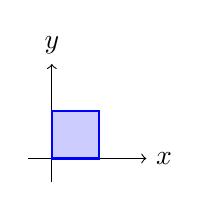
\begin{tikzpicture}[scale=0.6]
            \draw[->] (-0.5,0) -- (2,0) node[right] {$x$};
            \draw[->] (0,-0.5) -- (0,2) node[above] {$y$};
            \fill[blue!20] (0,0) rectangle (1,1);
            \draw[thick, blue] (0,0) rectangle (1,1);
        \end{tikzpicture}
        \caption{Item (11)}
    \end{subfigure}

    \vspace{0.6cm}

    % Item 12
    \begin{subfigure}[b]{0.3\linewidth}
        \centering
        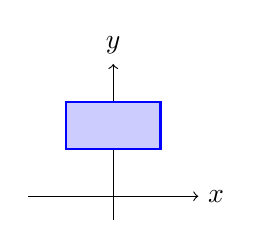
\begin{tikzpicture}[scale=0.6]
            \draw[->] (-1.8,0) -- (1.8,0) node[right] {$x$};
            \draw[->] (0,-0.5) -- (0,2.8) node[above] {$y$};
            \fill[blue!20] (-1,1) rectangle (1,2);
            \draw[thick, blue] (-1,1) rectangle (1,2);
        \end{tikzpicture}
        \caption{Item (12)}
    \end{subfigure}\hfill
    % Item 13
    \begin{subfigure}[b]{0.3\linewidth}
        \centering
        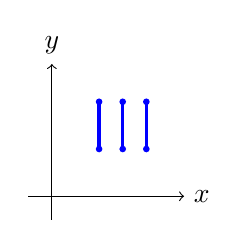
\begin{tikzpicture}[scale=0.6]
            \draw[->] (-0.5,0) -- (2.8,0) node[right] {$x$};
            \draw[->] (0,-0.5) -- (0,2.8) node[above] {$y$};
            \foreach \x in {1,1.5,2} {
                \draw[very thick, blue] (\x,1) -- (\x,2);
                \fill[blue] (\x,1) circle (2pt) (\x,2) circle (2pt);
            }
        \end{tikzpicture}
        \caption{Item (13)}
    \end{subfigure}\hfill
    % Item 14
    \begin{subfigure}[b]{0.3\linewidth}
        \centering
        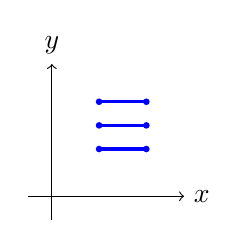
\begin{tikzpicture}[scale=0.6]
            \draw[->] (-0.5,0) -- (2.8,0) node[right] {$x$};
            \draw[->] (0,-0.5) -- (0,2.8) node[above] {$y$};
            \foreach \y in {1,1.5,2} {
                \draw[very thick, blue] (1,\y) -- (2,\y);
                \fill[blue] (1,\y) circle (2pt) (2,\y) circle (2pt);
            }
        \end{tikzpicture}
        \caption{Item (14)}
    \end{subfigure}

    \caption{Plots for Cartesian Products (Items 9--14)}\label{fig:cartesian_1}
\end{figure}

% --- SECOND PAGE: Items 15 to 20 ---
\begin{figure}[htbp]
    \ContinuedFloat%
    \centering
    % Item 15
    \begin{subfigure}[b]{0.3\linewidth}
        \centering
        \begin{tikzpicture}[scale=0.6]
            \draw[->] (-0.5,0) -- (2.2,0) node[right] {$x$};
            \draw[->] (0,-0.5) -- (0,2) node[above] {$y$};
            \draw[very thick, blue] (1,0) -- (1,1);
            \fill[blue] (1,0) circle (2pt) (1,1) circle (2pt);
        \end{tikzpicture}
        \caption{Item (15)}
    \end{subfigure}\hfill
    % Item 16
    \begin{subfigure}[b]{0.3\linewidth}
        \centering
        \begin{tikzpicture}[scale=0.6]
            \draw[->] (-0.5,0) -- (2,0) node[right] {$x$};
            \draw[->] (0,-0.5) -- (0,2) node[above] {$y$};
            \draw[very thick, blue] (0,1) -- (1,1);
            \fill[blue] (0,1) circle (2pt) (1,1) circle (2pt);
        \end{tikzpicture}
        \caption{Item (16)}
    \end{subfigure}\hfill
    % Item 17
    \begin{subfigure}[b]{0.3\linewidth}
        \centering
        \begin{tikzpicture}[scale=0.6]
            \draw[->] (-0.5,0) -- (3.2,0) node[right] {$x$};
            \draw[->] (0,-2.2) -- (0,2.2) node[above] {$y$};
            \foreach \x in {1,2,3} {
                \foreach \y in {-2,-1,0,1,2} {
                    \fill[blue] (\x,\y) circle (2pt);
                }
            }
            \node[blue] at (3.1, 0) {$\dots$};
            \node[blue] at (2, 2.1) {$\vdots$};
            \node[blue] at (2, -2.1) {$\vdots$};
        \end{tikzpicture}
        \caption{Item (17) $\mathbb{N} \times \mathbb{Z}$}
    \end{subfigure}

    \vspace{0.6cm}

    % Item 18
    \begin{subfigure}[b]{0.3\linewidth}
        \centering
        \begin{tikzpicture}[scale=0.6]
            \draw[->] (-2.2,0) -- (2.2,0) node[right] {$x$};
            \draw[->] (0,-2.2) -- (0,2.2) node[above] {$y$};
            \foreach \x in {-2,-1,0,1,2} {
                \foreach \y in {-2,-1,0,1,2} {
                    \fill[blue] (\x,\y) circle (2pt);
                }
            }
            \node[blue] at (2.1, 0) {$\dots$};
            \node[blue] at (-2.1, 0) {$\dots$};
            \node[blue] at (0, 2.1) {$\vdots$};
            \node[blue] at (0, -2.1) {$\vdots$};
        \end{tikzpicture}
        \caption{Item (18) $\mathbb{Z}^2$}
    \end{subfigure}\hfill
    % Item 19
    \begin{subfigure}[b]{0.3\linewidth}
        \centering
        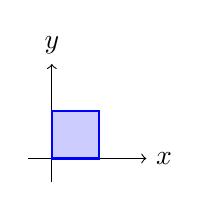
\begin{tikzpicture}[scale=0.6]
            \draw[->] (-0.5,0) -- (2,0) node[right] {$x$};
            \draw[->] (0,-0.5) -- (0,2) node[above] {$y$};
            \fill[blue!20] (0,0) rectangle (1,1);
            \draw[thick, blue] (0,0) rectangle (1,1);
        \end{tikzpicture}
        \caption{Item (19) $[0,1]{^2}$}
    \end{subfigure}\hfill
    % Item 20
    \begin{subfigure}[b]{0.3\linewidth}
        \centering
        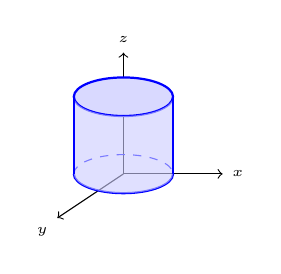
\begin{tikzpicture}[scale=0.7]
            % 3D Axes
            \draw[->] (0,0) -- (1.8,0) node[right] {\tiny $x$};
            \draw[->] (0,0) -- (0,2.2) node[above] {\tiny $z$};
            \draw[->] (0,0) -- (-1.2,-0.8) node[below left] {\tiny $y$};
            
            % Cylinder Body (Solid Disk x [0,1])
            \filldraw[fill=blue!15, draw=blue, thick] (0,1.4) ellipse (0.9cm and 0.35cm);
            \draw[thick, blue] (-0.9,0) arc (180:360:0.9cm and 0.35cm);
            \draw[dashed, blue] (-0.9,0) arc (180:0:0.9cm and 0.35cm);
            \fill[blue!20, opacity=0.6] (-0.9,0) arc (180:360:0.9cm and 0.35cm) -- (0.9,1.4) arc (0:-180:0.9cm and 0.35cm) -- cycle;
            \draw[thick, blue] (-0.9,0) -- (-0.9,1.4);
            \draw[thick, blue] (0.9,0) -- (0.9,1.4);
        \end{tikzpicture}
        \caption{Item (20) Disk $\times [0,1]$}
    \end{subfigure}

    \caption{Plots for Cartesian Products (Items 15--20, Continued)}\label{fig:cartesian_2}
\end{figure}
\end{solution}

\section{Solutions to Exercises from Section 3}
\begin{solution}\label{sol:3.1}\ref{ex:3.1}
    
    $$
    \begin{aligned}
        &(1)~ \{ 1,2,3,4 \}=\\
        &\varnothing, \{ 1 \},\{ 2 \},\{ 3 \},\{ 4 \},\\
        &\{ 1,2 \},\{ 1,3 \},\{ 1,4 \},\{ 2,3 \},\\
        &\{ 2,4 \}, \{ 3,4 \},\{ 1,2,3 \},\{ 1,2,4 \},\\
        &\{ 1,3,4 \}, \{ 2,3,4 \}, \{ 1,2,3,4 \}\\\\
        &(2)~\{ 1,2,\varnothing \}=\\
        &\varnothing, \{ 1 \},\{ 2\},\\
        &\{ \varnothing \}, \{ 1,2 \},\{ 1,\varnothing \},\\
        &\{ 2,\varnothing \}, \{ 1,2,\varnothing \}\\\\
        &(3)~ \{ \{ \R \} \}=\varnothing, \{ \R \}\\\\
        &(4)~\varnothing = \varnothing\\\\
        &(5)~\{ \varnothing \}=\varnothing, \{ \varnothing \}\\\\
        &(6)~\{ \R,\Q,\N \}=\\
        &\varnothing, \{ \R \},\{ N \},\{ \Q \},\\
        &\{ \R,\N \},\{ \R,\Q \}, \{ \N,\Q \},\{ \R,\N,\Q \}\\\\
        &(7)~\{ \R,\{ \N,\Q \} \}=\\
        &\varnothing, \{ \R \},\{\{ \N,\Q \}\}, \{ \R,\{ \N,\Q \} \}\\\\
        &(8)~\{ \{ 0,1 \},\{ 0,1,\{ 2 \} \},\{ 0 \} \}=\\
        &\varnothing, \{\{ 0,1 \}\}, \{\{ 0,1,\{ 2 \} \}\},\{\{ 0 \}\},\\
        &\{ \{ 0,1 \},\{ 0,1,\{ 2 \} \} \}, \{ \{ 0,1 \}, \{ 0 \} \},\\
        &\{ \{ 0,1,\{ 2 \} \},\{ 0 \} \}, \{ \{ 0,1 \},\{ 0,1,\{ 2 \} \},\{ 0 \} \}.
    \end{aligned}
    $$
\end{solution}

\begin{solution}\label{sol:3.2}\ref{ex:3.2}
    $$
    \begin{aligned}
    &(1)~\{ X:X\subseteq \{ 3,2,a \}\text{ and } \lvert X \rvert=2 \}=\{ \{ 3,2 \},\{ 3,a \},\{ 2,a \} \}\\\\
    &(2)~\{ X\subseteq\N:\lvert X \rvert\le 1 \}=\{ \varnothing \}\cup \{ \{ n \}:n\in\N \}\\\\
    &(3)~\{ X:X\subseteq \{ 3,2,a \}\text{ and }\lvert X \rvert=4 \}=\varnothing\\\\
    &(4)~\{ X:X\subseteq \{ 3,2,a \}\text{ and }\lvert X \rvert=1 \}=\{ \{ 3 \},\{ 2 \},\{ a \} \}\\\\
    \end{aligned}
    $$ 
   \end{solution}

\begin{solution}\label{sol:3.3}\ref{ex:3.3}
   
   $$
   (1)~\R^3\subseteq\R^3
   $$

   $(1)$ is true, for the fact that every set is a subset of itself. 
   
   $$
   (2)~\R^2\subseteq\R^3
   $$
   $(2)$ is tricky, strictly speaking it is false. However, if you have any experience with Linear Algebra you might consider it true. In Linear Algebra we abuse the notation and say that $\R^3$ is an extension of $\R^2$, addiing the third dimension to a two dimensional plane. In set theory however, we are a bit more strict. The above is false, since 
   $$
   \R^2=\R\times\R=\{ (x,y):x\in \R\land y\in\R \},
   $$
   And 
   $$
   \R^3=\R\times\R\times\R=\{ (x,y,z):x\in\R\land y\in\R \land z\in\R \}.
   $$
   So, the first \emph{object} takes in pairs, and the second object takes in triples. 

   $$
   (3)~\{ (x,y)\in\R^2:x-1=0 \}\subseteq \{ (x,y)\in\R^2:x^2-x=0 \}.
   $$
   Consider a small example here, the set contains pairs $(x,y)$, the first element of the pair has to be $1$, so $\{ (1,y):y\in\R \}$. In the second set we have $x^2-x=0$, solving this gives us $x=0,\lor x=1$, so we have the pairs $\{ (0,y),(1,y):y\in\R \}$. Then it follows that the example is true. 
   $$
   (4)~\{ (x,y)\in\R^2:x^2-x=0 \}\subseteq \{ (x,y)\in\R^2:x-1=0 \}.
   $$
   This example is false, in the LHS, we can have $0^2-0=0$, whereas in the RHS we cannot, unless $x=1$.  
\end{solution}
\section*{Solutions to Exercises from Section 4}
\begin{solution}\label{sol:4.1}\ref{ex:4.1}
    I will also show the cardinality of the powerset since I think it helps with counting all its subsets.
    $$
    \begin{aligned}
        &(1)~\powerset(\{\{ a,b \},\{ c \}\}) = \{ \varnothing,\{ \{ a,b \} \},\{ \{ c \} \},\{ \{ a,b \},\{ c \} \} \}\quad  \lvert \powerset(\{ \{ a,b \},\{ c \} \}) \rvert=2^2=4 \text{ elements}\\\\
        &(2)~\powerset(\{ 1,2,3,4 \})= \{ \varnothing,\{ 1 \},\{ 2 \},\{ 3 \},\{ 4 \},\\
        &\{ 1,2 \},\{ 1,3 \},\{ 1,4 \},\{ 2,3 \},\{ 2,4 \},\\
        &\{ 3,4 \},\{ 1,2,3 \},\{ 1,2,4 \},\{ 1,3,4 \},\{ 2,3,4 \},\{ 1,2,3,4 \} \}=2^4=16 \text{ elements}. \\\\
        &(3)~\powerset(\{ \{ \varnothing \},5 \})= \{ \varnothing,\{ \{ \varnothing \} \},\{ 5 \}, \{ \{ \varnothing \},5 \} \}=2^2=4 \text{ elements}.\\\\
        &(4)~ \powerset(\{ \R,\Q \})= \{ \varnothing, \{ \R \},\{ \Q \},\{ \R,\Q \} \}=2^2=4 \text{ elements}. \\\\
        &(5)~\powerset(\powerset(\{ 2 \}))=\powerset(\{ \varnothing, \{ 2 \} \})=\\
        &\{ \varnothing,\{ \varnothing \}, \{ \{ 2 \} \}, \{ \varnothing, \{ 2 \} \} \}=2^2=4 \text{ elements.}\\\\
        &(6)~\powerset(\{ 1,2 \})\times\powerset(\{ 3 \})=\\
        &\{ \varnothing,\{ 1 \},\{ 2 \},\{ 1,2 \} \}\times \{ \varnothing, \{ 3 \} \}=\\
        & \{ (\varnothing, \varnothing), (\varnothing, \{ 3 \}), (\{ 1 \},\varnothing), (\{ 1 \},\{ 3 \}),\\
        & (\{ 2 \},\varnothing),(\{ 2 \},\{ 3 \}), (\{ 1,2 \},\varnothing),(\{ 1,2 \},\{ 3 \}) \}\\\\
        &(7)~\powerset(\{ a,b \})\times\powerset(\{ 0,1 \})=\\
        & \{ \varnothing,\{ a \},\{ b \},\{ a,b \} \}\times \{ \varnothing,\{ 0 \},\{ 1 \},\{ 0,1 \} \}=\\
        & \{ (\varnothing,\varnothing), (\varnothing, \{ 0 \}),(\varnothing, \{ 1 \}),(\varnothing, \{ 0,1 \}),\\
        &(\{ a \},\varnothing),(\{ a \},\{ 0 \}),(\{ a \},\{ 1 \}),(\{ a \},\{ 0,1 \}),\\
        &(\{ b \},\varnothing),(\{ b \},\{ 0 \}),(\{ b \},\{ 1 \}), (\{ b \},\{ 0,1 \}),\\
        &(\{ a,b \},\varnothing),(\{ a,b \},\{ 0 \}),(\{ a,b \},\{ 1 \}),(\{ a,b \},\{ 0,1 \}) \}\\\\
        &(8)~\powerset(\{ 1,2 \}\times \{ 3 \})= \powerset(\{ (1,3),(2,3) \})=\\
        & \{ \varnothing, \{ (1,3) \},\{ (2,3) \},\{ (1,3),(2,3) \} \}\\\\
        &(9)~\powerset(\{ a,b \}\times \{ 0 \})=\powerset(\{ (a,0),(b,0) \})=\\
        &\{ \varnothing,\{ (a,0) \},\{ (b,0) \},\{ (a,0),(b,0) \} \}
    \end{aligned}
    $$
    We will do the last three examples separately, since there is a bit more to consider. Let's start with $(10)$:
    $$
    (10)~\{ X\in\powerset(\{ 1,2,3 \}): \lvert X \rvert\le 1 \}
    $$
    Notice that we are looking for a \emph{member} $X$, that has size no bigger than $1$. So, let's count the powerset and then see which sets qualify. 
    $$
    \begin{aligned}
        &\powerset(\{ 1,2,3 \})= \{ \varnothing, \{ 1 \},\{ 2 \},\{ 3 \},\\
        &\{ 1,2 \},\{ 1,3 \},\{ 2,3 \},\{ 1,2,3 \} \}=2^3=8 \text{elements}
    \end{aligned}
    $$
    Now, for the condition $X\in\powerset(\{ 1,2,3 \})$. We have 
    $$
    \{\varnothing, \{ 1 \},\{ 2 \},\{ 3 \}\}.
    $$
These are all the singletons and the empty set. For $(11)$, we have 
$$
\{ \varnothing,\{ \varnothing \}, \{ \{ 1 \} \},\{ \{ 2 \} \},\{ \{ 3 \} \}, \{ \{ 1,2 \} \},\{ \{ 1,3 \} \},\{ \{ 2,3 \} \},\{ \{ 1,2,3 \} \} \}.
$$
This might seem strange, but these are all of cardinality at most than $1$. Notice that the subsets of the powerset are all enclosed in an extra pair of curly braces, so they are counted as having one element. Lastly, for $(12)$ the condition changes slightly, we need to find $X\in\powerset(\{ 1,2,3 \})$ such that $2\in X$. So, 
$$
\{\{ 2 \},\{ 1,2 \},\{ 2,3 \},\{ 1,2,3 \}\}.
$$    
\end{solution}

\begin{solution}\label{sol:4.2}\ref{ex:4.2}
    We let $\lvert A \rvert= m ,\lvert B \rvert= n$, then 
    $$
    \begin{aligned}
        &(1)~\lvert \powerset\powerset\powerset(A) \rvert=2^{2^{2^{m}}}\\\\
        &(2)~\lvert \powerset\powerset(A) \rvert=2^{2^{m}}\\\\
        &(3)~\lvert \powerset(A\times B) \rvert=2^{m\cdot n}\\\\
        &(4)~\lvert \powerset(A)\times \powerset(B) \rvert=2^{m}\cdot 2^{n}\\\\
        &(5)~\lvert \{ X\in\powerset(A):\lvert X \rvert\le 1 \} \rvert= m+1\\\\
        &(6)~\lvert \powerset(A\times\powerset(B)) \rvert=2^{m\cdot 2^{n}}\\\\
        &(7)~ \lvert \powerset\powerset\powerset(A\times\varnothing) \rvert=4\\\\
        &(8)~\lvert \{ X\subseteq\powerset(A):\lvert X \rvert\le 1 \} \rvert=2^{m}+1.
    \end{aligned}
    $$
    \emph{Some Further Comments:} For $(5)$ it is important to understand the following. We are looking at members of the powerset, as in the previous exercise, we saw that these would be all the singletons and the empty set. Since we have exactly $m$ singletons and we add the empty set to that, so we get $m+1$. 
    Since the product of any set with the empty set is empty, we have to calculate $\lvert \powerset\powerset\powerset(\varnothing) \rvert$. The idea in $(8)$ is the same as in the previous exercise. 
\end{solution}

\section*{Solutions to Exercises from Section 5}
\begin{solution}\label{sol:5.1}\ref{ex:5.1}
    \begin{enumerate}
        \item $A\cup B=\{ 1,3,4,5,6,7,8,9 \}$
        \item $A\cap B=\{ 4,6 \}$
        \item $A-B=\{ 1,3,7,9 \}$
        \item $A-C=\{ 1,3,6,7,9 \}$
        \item $B-A=\{ 5,8 \}$
        \item $A\cap C=\{ 4 \}$
        \item $B\cap C=\{ 4,5,8 \}$
        \item $B\cup C=\{ 4,5,6,8 \}$
        \item $C-B=\varnothing$
    \end{enumerate}
\end{solution}

\begin{solution}\label{sol:5.2}\ref{ex:5.2}
    \begin{enumerate}
        \item $A\cup B=\{ 0,1,2,3,4,5,6,7,8 \}$
        \item $A\cap B=\varnothing$
        \item $A-B=A$ since $A\cap B=\varnothing$ (or in other words are disjoint)
        \item $A-C=\{ 0,6 \}$
        \item $B-A=B$ 
        \item $A\cap C=\{ 2,8,4 \}$
        \item $B\cap C=\varnothing$
        \item $B\cup C=\{ 1,2,3,4,5,7,8 \}$
        \item $C-B=C$
    \end{enumerate}
\end{solution}

\section{Solutions to Exercises from Section 6}

\begin{solution}\label{sol:6.1}\ref{ex:6.1}
    \begin{enumerate}
        \item $A^{\complement}=\{ 0,2,5,8,10 \}$
        \item $B^{\complement}=\{ 0,1,2,3,7,9,10 \}$
        \item $A\cap A^{\complement}=\{ 0,2,5,8,10 \}\cap \{ 4,3,6,7,1,9 \}=\varnothing$
        \item $A\cup A^{\complement}=U$ by the same logic as the above example
        \item $A-A^{\complement}=\{ 0,2,5,8,10 \}-\{ 4,3,6,7,1,9 \}=\{ 0,2,5,8,10 \}=A$
        \item $A-B^{\complement}=\{ 4,6 \}$
        \item $A^{\complement}-B^{\complement}=\{ 5,8 \}$
        \item $A^{\complement}\cap B=\{ 5,8 \}$
        \item ${(A^{\complement}-B)}^{\complement}=\{ 1,3,4,5,6,7,9 \}$
    \end{enumerate}
\end{solution}

\begin{solution}\label{sol:6.2}\ref{ex:6.2}
    \begin{enumerate}
        \item $A^{\complement}=\{ 1,3,5,7 \}=B$
        \item $B^{\complement}=\{ 0,2,4,6,8 \}=A$
        \item $A\cap A^{\complement}=\varnothing$
        \item $A\cup A^{\complement}=U$
        \item $A-A^{\complement}=A$
        \item ${(A\cup B)}^{\complement}=\varnothing$
        \item $A^\complement\cap B^{\complement}=\varnothing$
        \item ${(A\cap B)}^{\complement}=U$
        \item $A^{\complement}\times B=\{ (1,1),(1,3),(1,5),\dots \}=B^{2}$
    \end{enumerate}
\end{solution}

\begin{solution}\label{sol:6.3}\ref{ex:6.3}
    You can find the solution for this exercise below. 
    \begin{figure}[htbp]
    \centering
    % Drawing 1: The set X
    \begin{subfigure}[b]{0.32\linewidth}
        \centering
        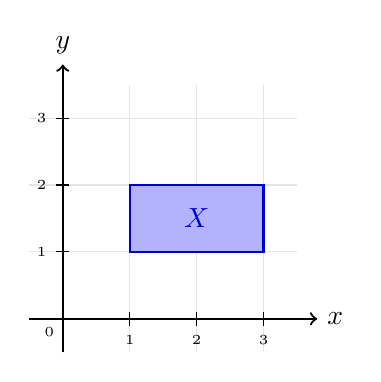
\begin{tikzpicture}[scale=0.85]
            % Grid & Axes
            \draw[gray!20, thin] (-0.5,-0.5) grid (3.5,3.5);
            \draw[->, thick] (-0.5,0) -- (3.8,0) node[right] {$x$};
            \draw[->, thick] (0,-0.5) -- (0,3.8) node[above] {$y$};
            
            % Ticks
            \foreach \x in {1,2,3} \draw (\x,0.1) -- (\x,-0.1) node[below] {\tiny $\x$};
            \foreach \y in {1,2,3} \draw (0.1,\y) -- (-0.1,\y) node[left] {\tiny $\y$};
            \node at (-0.2,-0.2) {\tiny $0$};

            % Set X: Shaded rectangle [1,3] x [1,2]
            \fill[blue!30] (1,1) rectangle (3,2);
            \draw[thick, blue!80!black] (1,1) rectangle (3,2);
            
            \node[blue!80!black] at (2,1.5) {$X$};
        \end{tikzpicture}
        \caption{The set $X = [1,3]\times[1,2]$}
    \end{subfigure}\hfill
    % Drawing 2: The set X^c
    \begin{subfigure}[b]{0.32\linewidth}
        \centering
        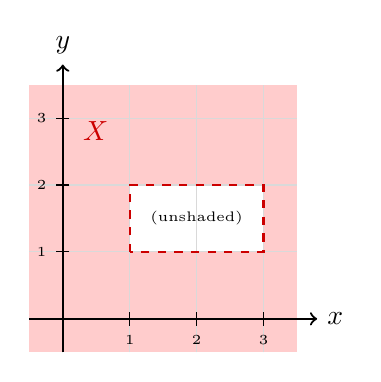
\begin{tikzpicture}[scale=0.85]
            % Outer shaded plane bounding box
            \fill[red!20] (-0.5,-0.5) rectangle (3.5,3.5);
            
            % Unshade the "hole" X
            \fill[white] (1,1) rectangle (3,2);
            
            % Grid & Axes
            \draw[gray!30, thin] (-0.5,-0.5) grid (3.5,3.5);
            \draw[->, thick] (-0.5,0) -- (3.8,0) node[right] {$x$};
            \draw[->, thick] (0,-0.5) -- (0,3.8) node[above] {$y$};
            
            % Ticks
            \foreach \x in {1,2,3} \draw (\x,0.1) -- (\x,-0.1) node[below] {\tiny $\x$};
            \foreach \y in {1,2,3} \draw (0.1,\y) -- (-0.1,\y) node[left] {\tiny $\y$};
            
            % Boundary of hole X
            \draw[thick, dashed, red!80!black] (1,1) rectangle (3,2);
            
            \node[red!80!black] at (0.5,2.8) {$X^{\complement}$};
            \node at (2,1.5) {\tiny (unshaded)};
        \end{tikzpicture}
        \caption{The complement $X^{\complement}$}
    \end{subfigure}\hfill
    % Drawing 3: X^c \cap ([0,2] \times [0,3])
    \begin{subfigure}[b]{0.32\linewidth}
        \centering
        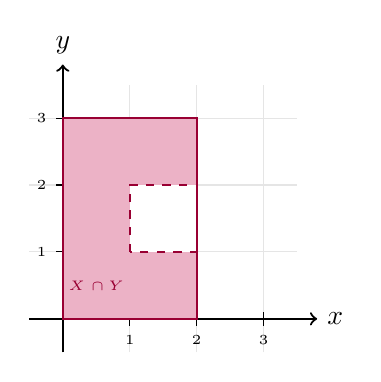
\begin{tikzpicture}[scale=0.85]
            % Grid & Axes
            \draw[gray!20, thin] (-0.5,-0.5) grid (3.5,3.5);
            \draw[->, thick] (-0.5,0) -- (3.8,0) node[right] {$x$};
            \draw[->, thick] (0,-0.5) -- (0,3.8) node[above] {$y$};
            
            % Ticks
            \foreach \x in {1,2,3} \draw (\x,0.1) -- (\x,-0.1) node[below] {\tiny $\x$};
            \foreach \y in {1,2,3} \draw (0.1,\y) -- (-0.1,\y) node[left] {\tiny $\y$};
            
            % Full region [0,2] x [0,3] shaded
            \fill[purple!30] (0,0) rectangle (2,3);
            % Hole where X overlaps: [1,2] x [1,2]
            \fill[white] (1,1) rectangle (2,2);
            
            % Outer boundary of [0,2] x [0,3]
            \draw[thick, purple!80!black] (0,0) rectangle (2,3);
            % Boundary of the removed hole
            \draw[thick, dashed, purple!80!black] (1,1) rectangle (2,2);
            
            \node[purple!80!black, font=\tiny] at (0.5,0.5) {$X^{\complement} \cap Y$};
        \end{tikzpicture}
        \caption{$X^{\complement}\cap([0,2]\times[0,3])$}
    \end{subfigure}

    \caption{Sketches of $X$, its complement $X^{\complement}$, and the restricted intersection.}\label{fig:ex_6_3}
\end{figure}
\end{solution}

\begin{solution}\label{sol:6.4}\ref{ex:6.4}
    Ditto.

    \begin{figure}[htbp]
    \centering
    % Drawing 1: The set X
    \begin{subfigure}[b]{0.32\linewidth}
        \centering
        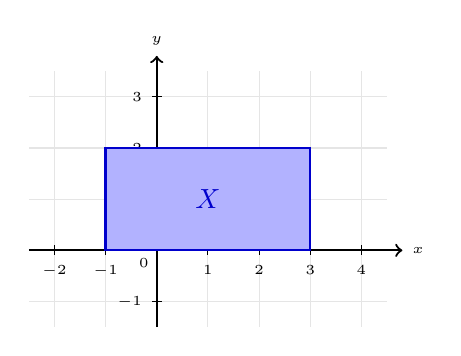
\begin{tikzpicture}[scale=0.65]
            % Grid & Axes
            \draw[gray!20, thin] (-2.5,-1.5) grid (4.5,3.5);
            \draw[->, thick] (-2.5,0) -- (4.8,0) node[right] {\tiny $x$};
            \draw[->, thick] (0,-1.5) -- (0,3.8) node[above] {\tiny $y$};
            
            % Ticks
            \foreach \x in {-2,-1,1,2,3,4} \draw (\x,0.1) -- (\x,-0.1) node[below] {\tiny $\x$};
            \foreach \y in {-1,1,2,3} \draw (0.1,\y) -- (-0.1,\y) node[left] {\tiny $\y$};
            \node at (-0.25,-0.25) {\tiny $0$};

            % Set X: Shaded rectangle [-1,3] x [0,2]
            \fill[blue!30] (-1,0) rectangle (3,2);
            \draw[thick, blue!80!black] (-1,0) rectangle (3,2);
            
            \node[blue!80!black] at (1,1) {$X$};
        \end{tikzpicture}
        \caption{The set $X$}
    \end{subfigure}\hfill
    % Drawing 2: The set X^c
    \begin{subfigure}[b]{0.32\linewidth}
        \centering
        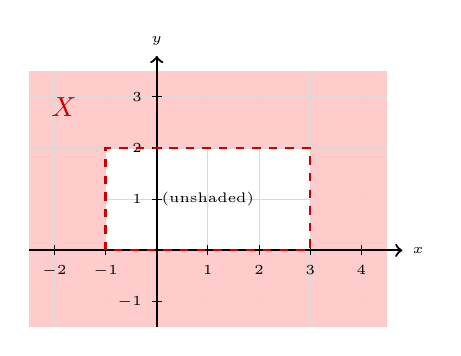
\begin{tikzpicture}[scale=0.65]
            % Outer shaded plane bounding box
            \fill[red!20] (-2.5,-1.5) rectangle (4.5,3.5);
            
            % Unshade the "hole" X
            \fill[white] (-1,0) rectangle (3,2);
            
            % Grid & Axes
            \draw[gray!30, thin] (-2.5,-1.5) grid (4.5,3.5);
            \draw[->, thick] (-2.5,0) -- (4.8,0) node[right] {\tiny $x$};
            \draw[->, thick] (0,-1.5) -- (0,3.8) node[above] {\tiny $y$};
            
            % Ticks
            \foreach \x in {-2,-1,1,2,3,4} \draw (\x,0.1) -- (\x,-0.1) node[below] {\tiny $\x$};
            \foreach \y in {-1,1,2,3} \draw (0.1,\y) -- (-0.1,\y) node[left] {\tiny $\y$};
            
            % Boundary of hole X
            \draw[thick, dashed, red!80!black] (-1,0) rectangle (3,2);
            
            \node[red!80!black] at (-1.8,2.8) {$X^{\complement}$};
            \node at (1,1) {\tiny (unshaded)};
        \end{tikzpicture}
        \caption{The complement $X^{\complement}$}
    \end{subfigure}\hfill
    % Drawing 3: X^c \cap ([-2,4] \times [-1,3])
    \begin{subfigure}[b]{0.32\linewidth}
        \centering
        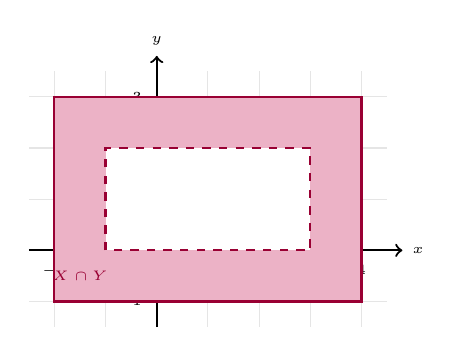
\begin{tikzpicture}[scale=0.65]
            % Grid & Axes
            \draw[gray!20, thin] (-2.5,-1.5) grid (4.5,3.5);
            \draw[->, thick] (-2.5,0) -- (4.8,0) node[right] {\tiny $x$};
            \draw[->, thick] (0,-1.5) -- (0,3.8) node[above] {\tiny $y$};
            
            % Ticks
            \foreach \x in {-2,-1,1,2,3,4} \draw (\x,0.1) -- (\x,-0.1) node[below] {\tiny $\x$};
            \foreach \y in {-1,1,2,3} \draw (0.1,\y) -- (-0.1,\y) node[left] {\tiny $\y$};
            
            % Full region [-2,4] x [-1,3] shaded
            \fill[purple!30] (-2,-1) rectangle (4,3);
            % Hole where X overlaps: [-1,3] x [0,2]
            \fill[white] (-1,0) rectangle (3,2);
            
            % Outer boundary of [-2,4] x [-1,3]
            \draw[thick, purple!80!black] (-2,-1) rectangle (4,3);
            % Boundary of the removed hole
            \draw[thick, dashed, purple!80!black] (-1,0) rectangle (3,2);
            
            \node[purple!80!black, font=\tiny] at (-1.5,-0.5) {$X^{\complement} \cap Y$};
        \end{tikzpicture}
        \caption{$X^{\complement}\cap([-2,4]\times[-1,3])$}
    \end{subfigure}

    \caption{Sketches for Exercise 6.4.}\label{fig:ex_6_4}
\end{figure}
\end{solution}

\begin{solution}\label{sol:6.5}\ref{ex:6.5}
    Ditto.
    \begin{figure}[htbp]
    \centering
    % Drawing 1: The set X (Annulus)
    \begin{subfigure}[b]{0.45\linewidth}
        \centering
        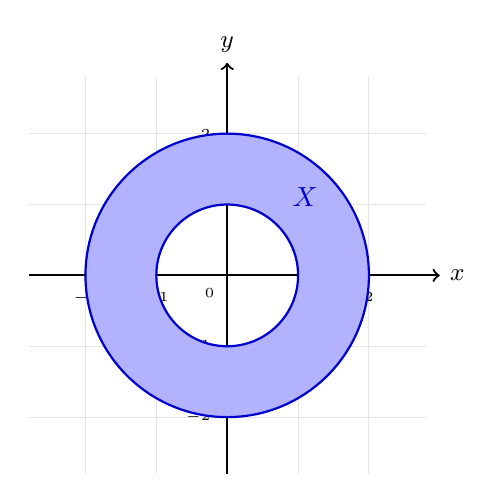
\begin{tikzpicture}[scale=0.9]
            % Grid & Axes
            \draw[gray!20, thin] (-2.8,-2.8) grid (2.8,2.8);
            \draw[->, thick] (-2.8,0) -- (3.0,0) node[right] {\small $x$};
            \draw[->, thick] (0,-2.8) -- (0,3.0) node[above] {\small $y$};
            
            % Ticks
            \foreach \x in {-2,-1,1,2} \draw (\x,0.1) -- (\x,-0.1) node[below] {\tiny $\x$};
            \foreach \y in {-2,-1,1,2} \draw (0.1,\y) -- (-0.1,\y) node[left] {\tiny $\y$};
            \node at (-0.25,-0.25) {\tiny $0$};

            % Shaded Annulus: Outer circle radius 2 minus inner circle radius 1
            \fill[blue!30, even odd rule] (0,0) circle (2cm) (0,0) circle (1cm);
            
            % Solid Boundaries
            \draw[thick, blue!80!black] (0,0) circle (2cm);
            \draw[thick, blue!80!black] (0,0) circle (1cm);
            
            \node[blue!80!black] at (1.1,1.1) {$X$};
        \end{tikzpicture}
        \caption{The set $X$ (Annulus $1 \le r \le 2$)}
    \end{subfigure}\qquad
    % Drawing 2: The Complement X^c
    \begin{subfigure}[b]{0.45\linewidth}
        \centering
        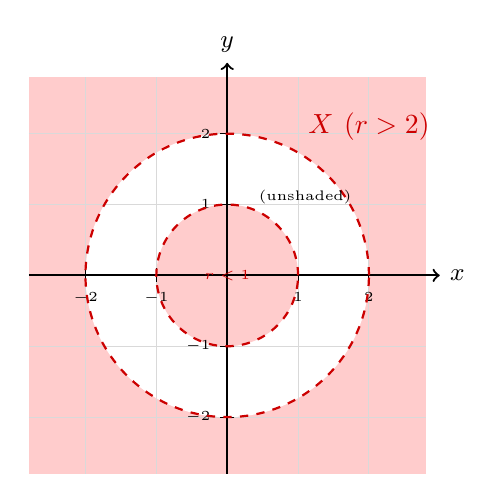
\begin{tikzpicture}[scale=0.9]
            % Outer bounding region shaded
            \fill[red!20] (-2.8,-2.8) rectangle (2.8,2.8);
            
            % Unshade the annulus X
            \fill[white] (0,0) circle (2cm);
            
            % Re-shade the inner core disk r < 1
            \fill[red!20] (0,0) circle (1cm);
            
            % Grid & Axes
            \draw[gray!30, thin] (-2.8,-2.8) grid (2.8,2.8);
            \draw[->, thick] (-2.8,0) -- (3.0,0) node[right] {\small $x$};
            \draw[->, thick] (0,-2.8) -- (0,3.0) node[above] {\small $y$};
            
            % Ticks
            \foreach \x in {-2,-1,1,2} \draw (\x,0.1) -- (\x,-0.1) node[below] {\tiny $\x$};
            \foreach \y in {-2,-1,1,2} \draw (0.1,\y) -- (-0.1,\y) node[left] {\tiny $\y$};
            
            % Dashed boundaries excluded from X^c
            \draw[thick, dashed, red!80!black] (0,0) circle (2cm);
            \draw[thick, dashed, red!80!black] (0,0) circle (1cm);
            
            \node[red!80!black] at (0,0) {\tiny $r < 1$};
            \node[red!80!black] at (2.0,2.1) {$X^{\complement}$ ($r > 2$)};
            \node at (1.1,1.1) {\tiny (unshaded)};
        \end{tikzpicture}
        \caption{The complement $X^{\complement}$ ($r < 1 \cup r > 2$)}
    \end{subfigure}

    \caption{Sketches for Exercise 6.5.}\label{fig:ex_6_5}
\end{figure}
\end{solution}

\begin{solution}\label{sol:6.6}\ref{ex:6.6}
    Ditto.
    
    \begin{figure}[htbp]
    \centering
    % Drawing 1: The set X (y < x^2)
    \begin{subfigure}[b]{0.45\linewidth}
        \centering
        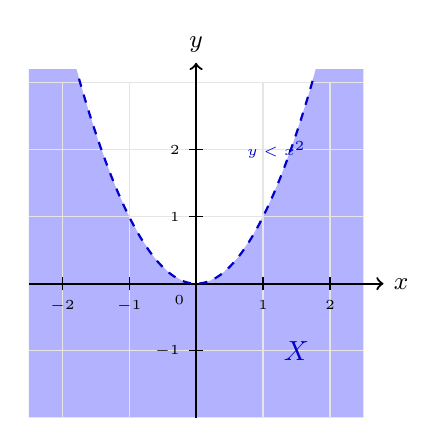
\begin{tikzpicture}[scale=0.85]
            % Bounding area for clip
            \begin{scope}
                \clip (-2.5,-2.0) rectangle (2.5,3.2);
                
                % Fill region below parabola y < x^2
                \fill[blue!30] plot[domain=-2.5:2.5, variable=\x] (\x, {\x*\x}) -- (2.5,-2.0) -- (-2.5,-2.0) -- cycle;
            \end{scope}

            % Grid & Axes
            \draw[gray!20, thin] (-2.5,-2.0) grid (2.5,3.0);
            \draw[->, thick] (-2.5,0) -- (2.8,0) node[right] {\small $x$};
            \draw[->, thick] (0,-2.0) -- (0,3.3) node[above] {\small $y$};
            
            % Ticks
            \foreach \x in {-2,-1,1,2} \draw (\x,0.1) -- (\x,-0.1) node[below] {\tiny $\x$};
            \foreach \y in {-1,1,2} \draw (0.1,\y) -- (-0.1,\y) node[left] {\tiny $\y$};
            \node at (-0.25,-0.25) {\tiny $0$};

            % Dashed parabola boundary y = x^2
            \draw[thick, dashed, blue!80!black, domain=-1.75:1.75, variable=\x, samples=100] plot (\x, {\x*\x});
            
            \node[blue!80!black] at (1.5,-1.0) {$X$};
            \node[blue!80!black, font=\tiny] at (1.2,2.0) {$y < x^2$};
        \end{tikzpicture}
        \caption{The set $X = \{(x,y) \in \mathbb{R}^2 : y < x^2\}$}
    \end{subfigure}\qquad
    % Drawing 2: The Complement X^c (y >= x^2)
    \begin{subfigure}[b]{0.45\linewidth}
        \centering
        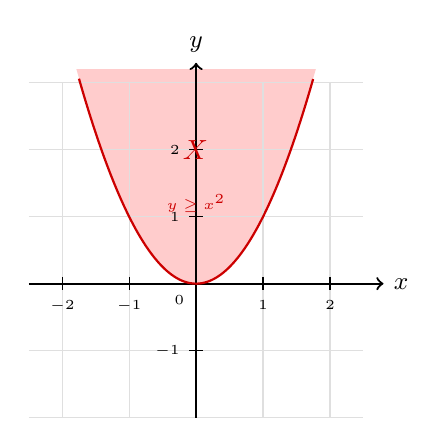
\begin{tikzpicture}[scale=0.85]
            % Bounding area for clip
            \begin{scope}
                \clip (-2.5,-2.0) rectangle (2.5,3.2);
                
                % Fill region on/above parabola y >= x^2
                \fill[red!20] plot[domain=-2.0:2.0, variable=\x] (\x, {\x*\x}) -- (2.5,3.5) -- (-2.5,3.5) -- cycle;
            \end{scope}

            % Grid & Axes
            \draw[gray!25, thin] (-2.5,-2.0) grid (2.5,3.0);
            \draw[->, thick] (-2.5,0) -- (2.8,0) node[right] {\small $x$};
            \draw[->, thick] (0,-2.0) -- (0,3.3) node[above] {\small $y$};
            
            % Ticks
            \foreach \x in {-2,-1,1,2} \draw (\x,0.1) -- (\x,-0.1) node[below] {\tiny $\x$};
            \foreach \y in {-1,1,2} \draw (0.1,\y) -- (-0.1,\y) node[left] {\tiny $\y$};
            \node at (-0.25,-0.25) {\tiny $0$};

            % Solid parabola boundary y = x^2
            \draw[thick, red!80!black, domain=-1.75:1.75, variable=\x, samples=100] plot (\x, {\x*\x});
            
            \node[red!80!black] at (0,2.0) {$X^{\complement}$};
            \node[red!80!black, font=\tiny] at (0,1.2) {$y \ge x^2$};
        \end{tikzpicture}
        \caption{The complement $X^{\complement} = \{(x,y) \in \mathbb{R}^2 : y \ge x^2\}$}
    \end{subfigure}

    \caption{Sketches for Exercise 6.6.}\label{fig:ex_6_6}
\end{figure}
\end{solution}
\section{Solutions to Exercises from Section 7}

Skipped.


\section{Solutions to Exercises from Section 8}

\begin{solution}\label{sol:8.1}\ref{ex:8.1}
    Let $A_{1}=\{ a,b,d,e,g,f \},A_{2}=\{ a,b,c,d \},A_{3}=\{ b,d,a \},A_{4}=\{ a,b,h \}$. Then,
    $$
    (1)~ \bigcup^{4}_{i=1}A_{i}= A_{1}\cup A_{2} \cup A_{3} \cup A_{4}=\{ a,b,c,d,e,f,g,h \}
    $$
    and 
    $$
    (2)~ \bigcap^{4}_{i=1}A_{i}=A_1 \cap A_2 \cap A_3 \cap A_4 =\{ a,b \}.
    $$
\end{solution}


\begin{solution}\label{sol:8.2}\ref{ex:8.2}
    Let $A_1= \{ 0,2,4,\dots,24 \},A_2=\{ 0,3,6,\dots,24 \},A_3=\{ 0,4,8,\dots,24 \}$. Then, 
    $$
    (1)~ \bigcup^{3}_{i=1}A_i=\{ 0,2,3,4,6,9,\dots,24 \}
    $$
    and 
    $$
    (2)~\bigcap^{3}_{i=1}A_i=\{ 0,12,14 \}.
    $$
\end{solution}


\begin{solution}\label{sol:8.3}\ref{ex:8.3}
    For each $n\in\N$, we let $A_n=\{ 0,1,2,3,4,\dots,n \}$. Let us first unpack what this means. Consider the following two interpretations: 
    $$
    A_0=\{ 0 \}, A_{1}=\{ 0,1 \},\dots \quad\quad A_1=\{ 0,1 \},A_2=\{ 0,1,2 \},\dots
    $$
    It is up to convention whether $\N=\{ 0,1,2,3,\dots \}$ or $\N=\{ 1,2,3,\dots \}$. Depending on the convention the answer might differ slightly. 
    Case $1$: 
    $$
    (1)~ \bigcup_{i\in\N}A_i= \N
    $$
    Case $2$: 
    $$
    (1)~ \bigcup_{i\in\N}A_i= \N\cup \{ 0 \}.
    $$
    Similarly for the second subpoint. 
    Case $1$: 
    $$
    (2)~ \bigcap_{i\in\N}A_i=\{ 0,1 \}
    $$
    and Case $2$:
    $$
    (2)~ \bigcap_{i\in\N}A_i=\{ 0 \}
    $$
\end{solution}

\begin{solution}\label{sol:8.4}\ref{ex:8.4}
    Let each $n\in \N$ with $A_{n} = \{ -2n, 0, 2n \}$, then similarly to before, we have 
    $$
    A_0 = \{ -2(0), 0, 2(0) \} \quad\quad A_1=\{ -2(1), 0, 2(1) \}, A_2=\{ -2(2), 0, 2(2) \}
    $$
    So, 
    $$
    \bigcup_{i\in\N}A_{i} = \{ \dots,-6,-4,-2,0,2,4,6,\dots \}
    $$
    and 
    $$
    \bigcap_{i\in\N}A_{i} = \{ 0 \}
    $$
    Similarly to before, if we assume that $\N=\N - \{ 0 \}$, then we will start from $A_1$ but this exercise will not be affected by that convetion like the previous one.
\end{solution}


\begin{solution}\label{sol:8.5}\ref{ex:8.5}
    
    $$
    (1)~ \bigcup_{i\in\N}[i,i+1]=[0,\infty)
    $$
    Here we assume that $0\in\N$, if you choose to assume the contrary, then the interval would start with $1$ instead of $0$.
    $$
    (2)~\bigcap_{i\in\N}[i,i+1]=\varnothing
    $$
    Since some pairs of intervals are disjoint ($[0,1]\cap[2,3]$). 
\end{solution}


\begin{solution}\label{sol:8.6}\ref{ex:8.6}
    $$
    (1)~\bigcup_{i\in\N}[0,i+1]=[0,\infty)
    $$
    and 
    $$
    (2)~\bigcap_{i\in\N}[0,i+1]=[0,1] \text{ or } [0,2] \text{ depending on whether we include } 0\in\N
    $$
\end{solution}


\begin{solution}\label{sol:8.7}\ref{ex:8.7}
    
    $$
    (1)~\bigcup_{i\in\N}\R\times[i,i+1]=\R\times [0,\infty)
    $$
    Again, in the above, convention matters, it will be the differnece between $[1,\infty)$ and the answer provided above. 
    $$
    (2)~\bigcap_{i\in\N}\R\times[i,i+1]=\varnothing
    $$
\end{solution}


\begin{solution}\label{sol:8.8}\ref{ex:8.8}
    
    $$
    (1)~\bigcup_{a\in\R}\{ a \}\times[0,1]=\R \times [0,1]
    $$
    We know that $a\in\R$ means that $a$ is any real number such that $\sqrt2\times[0,1]$ for example. 
    $$
    (2)~\bigcap_{a\in\R}\{ a \}\times[0,1]=\varnothing
    $$
\end{solution}


\begin{solution}\label{sol:8.9}\ref{ex:8.9}
    
    $$
    (1)~\bigcup_{X\in\powerset(\N)}X=\N
    $$
    The way to think about it is that because $X\in\powerset(\N)$, then $X$ can be any subset of the natural numbers. The union of those subsets would be the natural numbers. 
    $$
    (2)~\bigcap_{X\in\powerset(\N)}X=\varnothing
    $$
    Important here is to remember that the empty set is part of $\powerset(\N)$.
\end{solution}

\begin{solution}\label{sol:8.10}\ref{ex:8.10}
    
    $$
    (1)~\bigcup_{x\in[0,1]}[x,1]\times[0,x^{2}]=\{ (u,v):0\le u\le 1, 0\le v \le u^{2} \}
    $$
    and 
    $$
    (2)~\bigcap_{x\in[0,1]}[x,1]\times[0,x^{2}]=\{ (1,0) \}
    $$
\end{solution}


\begin{solution}\label{sol:8.11}\ref{ex:8.11}
    Yes, this is always true. Informally speaking, the intersection of two sets is almost always smaller than their union. Consider the example: 
    $$
    \{ 1,2,3 \}\cup \{ 2,3,4 \}= \{ 1,2,3,4 \} \quad\quad \{ 1,2,3 \}\cap \{ 2,3,4 \}=\{ 2,3 \}.
    $$
    In the case when the intersection is empty and the two sets disjoint, then we know that the empty set is a subset of any set, so the statement still holds. 

    For a more formal proof, let $\alpha\in I$, then suppose for some $x\in\alpha_{0}$. Since, $x\in\alpha_{0}$ and $\alpha\in I$, then $x\in A_{\alpha_{0}}$. Therefore, $x\in\bigcup_{\alpha\in I}A_{\alpha}$.
\end{solution}

\begin{solution}\label{sol:8.12}\ref{ex:8.12}
    Now we consider the relationship between $\bigcap_{\alpha\in I}A_{\alpha}=\bigcup_{\alpha\in I}A_{\alpha}$. Clearly if they are equal the first thing to consider would be that two sets are equal, meaning 
    $$
    \{ 1,2,3 \}\cap \{ 1,2,3 \}=\{ 1,2,3 \} \quad\quad \{ 1,2,3 \}\cup \{ 1,2,3 \}=\{ 1,2,3 \}
    $$
    In other words, that all $A_{\alpha}$ are equal. 
\end{solution}

\begin{solution}\label{sol:8.13}\ref{ex:8.13}
    If $J\ne\varnothing, J\subseteq I$, then is it true that $\bigcup_{\alpha\in J}A_{\alpha}\subseteq \bigcup_{\alpha\in I}A_{\alpha}$? Let us break down the statement. First, suppose that $J=\{ 1,2,3 \}$ and $I=\{ 1,2,3,4 \}$, then the statement would be true. Intuitively, the idea is that $J$ can be at most as large as $I$. If we think about the definition of big union 
    $$
    \bigcup_{\alpha\in J}A_\alpha=\{ x: \exists \alpha \in I, x\in A_\alpha \},
    $$
    so, the requirement is that at \emph{at least one} $x$ that is a member of $A_{\alpha}$, then since $J\subseteq I$, it follows by definition of subsets that the equivalence holds. 
    
    Now, let's consider the second one. The definition of big intersection is $\forall \alpha \in I, x\in A_{\alpha}$ to be true. This however is not necessitated by the definition of subets. So it could be true, but it \emph{does not} hold in general. 
\end{solution}

\begin{solution}\label{sol:8.14}\ref{ex:8.14}
    If $J\ne\varnothing,J\subseteq I$, then $\bigcap_{\alpha\in I}A_{\alpha}\subseteq \bigcap_{\alpha \in J}A_{\alpha}$. Now, let some arbitrary element $x\in \bigcap_{\alpha\in I}A_{\alpha}$, then $\forall \alpha \in I, x\in A_{\alpha}$. Similar to before, if $J\subseteq I$, then $J$ is at most as big as $I$. Since, all $x\in A_{\alpha}$ for an arbitrary $x$, then it follows that $\forall \alpha \in J, x \in A_{\alpha}$. Thus, $x\in\bigcap_{\alpha\in J}A_{\alpha}$.
\end{solution}

%Solutions from Chapter 2
\section*{Solutions to Exercises From Section 11}
\begin{solution}\label{sol:2.11}\ref{ex:2.11}
    \begin{enumerate}
        \item This is a false statement. 
        \item This is a true statement. 
        \item This is a true statement. 
        \item This is not a statement. 
        \item This is a true statement. 
        \item This is a true statement. 
        \item This is a false statement. 
        \item This is a false statement. 
        \item This is an open sentence/formula. 
        \item This is a true statement. 
        \item This is an open sentence/formula. 
        \item This is a true statement. It is called a \emph{tautology}.
        \item This is a true statement. 
        \item This is not a statement. 
        \item This is technically a statement since it can be either true or false. But its truth value is unclear. It is similar to a conjecture. 
    \end{enumerate}
\end{solution}

\section{Solutions to Exercises From Section 12}
\begin{solution}\label{sol:2.12}\ref{ex:2.12}
    \begin{enumerate}
        \item $P$: `The number $8$ is even', $Q$: `The number $8$ is a power of $2$', so $P\land Q$. 
        \item $P$: The matrix $A$ is invertible. Then $\neg P$. 
        \item $x\ne y$ is the same as $\neg(x=y)$, so if $P:x=y$, then $\neg P:x\ne y$. 
        \item $x < y$ is the same as $\ne(x\ge y)$, so similarly to above we have $\neg P$, where $P$ is $x\ge y$. 
        \item $y\ge x$ is equivalent to $\neg(y<x)$, so again we can simply state $\neg P$, where $P$ is $y<x$. 
        \item $P$: Scheduled for Wednesday, $Q$: Scheduled for Friday, so $P\lor Q$.\footnote{When we later look at quantifiers and predicates, we will find that there is another more expressive way to represent the above statement: $\exists x(P(x)\lor Q(x))$ where $x$ represents the quiz. Furthermore, we can say that there is a quiz on Wednesday or Friday but not both days: $\exists x((P(x)\lor Q(x))\land \neg(P(x)\land Q(x)))$.}
        \item $P:x=0$ and $Q:y=0$ so, $P\land\neg Q$. 
        \item $P:x=0$ and $Q:y=0$, so $P\lor Q$. Similarly, to the footnote, we can transform this accordingly with predicates and quantifiers. 
        \item $x\in A\land x\notin B$.
        \item $x\in A\lor x\in B$.
        \item This one is slightly trickier. Let $A$ be a member of the set, then $A\in\powerset(\N)$, so now we have to `append' the condition on $A$, which is $\lvert A^{\complement} \rvert<\infty$, so together we have $A\in\powerset(\N)\land \lvert A^{\complement} \rvert<\infty$.
        \item $H$: Happy families, $A$: Alike, $W$: Unhappy in its own way. Breaking down the statement we have, if a family is happy, then it is alike, \emph{and} if it is not happy, then it is unhappy in its own way. Therefore, $(H\Rightarrow A)\land(\neg H\Rightarrow W)$. If we don't want to use arrows or conditional statements, the formula looks thus: $(\neg H\lor A)\land (H\lor W)$.
        \item $H$: Human beings want to be good, $S$: Too good, $R$: All the time. So, $H\land \neg S \land \neg R$. 
        \item $P$: A man should look for what is, $Q$: A man should look for what he think should be. Then, $P\land \neg Q$.
    \end{enumerate}
\end{solution}
\section*{Solutions for Exercises from Section 13}
\begin{solution}\label{sol:2.13}\ref{ex:2.13}
    \begin{enumerate}
        \item If the determinant is not zero, then the matrix is invertible. 
        \item If a function is differentiable, then it is continuous. 
        \item If a function is continuous, then it is integrable. 
        \item If a function is a polynomial, then it is rational. 
        \item If an integer is divisible by $8$, then it is divisible by $4$. 
        \item If a surface has only one side, then it is non-orientable. 
        \item If a series converges absolutely, then it converges. 
        \item If the ratio $r$ of a geometric series is $\lvert r \rvert<1$, then the series converges. 
        \item If a function is continuous, then the function is also integrable. 
        \item If the descriminant is negative, then the quadratic equation has no real solutions. 
        \item If you stop writing, you fail. 
        \item In general, if people accept facts as truth, then the facts agree with what they already believe. 
        \item If people agree with me, then I feel I must be wrong. 
    \end{enumerate}
\end{solution}
\section*{Solutions to Exercises from Section 14}
\begin{solution}\label{sol:2.14}\ref{ex:2.14}
    \begin{itemize}
        \item A matrix $A$ is invertible if and only if (iff) $\det(A)\ne 0$.
        \item A function has a constant derivative iff it is linear. 
        \item $xy=0$ iff $x=0$ or $y=0$. 
        \item $a\in\Q$ iff $5a\in\Q$. 
        \item An occurrence is an adventure iff one recounts it.
    \end{itemize}
\end{solution}
\section*{Solutions for Exercises from Section 15}
\begin{solution}\label{sol:2.15.1}\ref{ex:2.15.1}
    For $(1)$: 
    \begin{table}[H]
    \centering
    \begin{tabular}{ccccc}
    \toprule
    $P$ & $Q$ & $R$ & $Q \Rightarrow R$ & $P \lor (Q \Rightarrow R)$ \\
    \midrule
    T & T & T & T & T \\
    T & T & F & F & T \\
    T & F & T & T & T \\
    T & F & F & T & T \\
    F & T & T & T & T \\
    F & T & F & F & \textbf{F} \\
    F & F & T & T & T \\
    F & F & F & T & T \\
    \bottomrule
    \end{tabular}
    \end{table}

    $(2)$:
    \begin{table}[H]
        \centering
        \begin{tabular}{ccc}
        \toprule
        $Q$ & $R$ & $(Q\lor R)\Leftrightarrow (R\land Q)$\\
        \midrule
        T & T & T\\
        T & F & F\\
        F & T & F\\
        F & F & T\\
        \bottomrule
        \end{tabular}
    \end{table}    
   
    $(3)$:
    \begin{table}[H]
        \centering
        \begin{tabular}{ccc}
            \toprule
            $P$ & $Q$ & $\neg(P\Rightarrow Q)$\\
            \midrule
            T & T & F \\
            T & F & T \\
            F & T & F \\
            F & F & F\\
            \bottomrule
        \end{tabular}
    \end{table}

    $(4)$:
    \begin{table}[H]
        \centering
        \begin{tabular}{ccc}
            \toprule
            $P$ & $Q$ & $\neg(P\lor Q)\lor(\neg P)$\\
            \midrule
            T & T & F\\
            T & F & F\\
            F & T & T\\
            F & F & T\\
            \bottomrule
        \end{tabular}
    \end{table}

    $(5)$:
        \begin{table}[H]
        \centering
        \begin{tabular}{ccc}
            \toprule
            $P$ & $Q$ & $(P\land\neg P)\lor Q$\\
            \midrule
            T & T & T\\
            T & F & F\\
            F & T & T\\
            F & F & F\\
            \bottomrule
        \end{tabular}
    \end{table}

    $(6)$: 
        \begin{table}[H]
        \centering
        \begin{tabular}{ccc}
            \toprule
            $P$ & $Q$ & $(P\land \neg P)\land Q$\\
            \midrule
            T & T & F\\
            T & F & F\\
            F & T & F\\
            F & F & F\\
            \bottomrule
        \end{tabular}
    \end{table}

    $(7)$:
        \begin{table}[H]
        \centering
        \begin{tabular}{ccc}
            \toprule
            $P$ & $Q$ & $\neg(P\land \neg P)\Rightarrow Q$\\
            \midrule
            T & T & T\\
            T & F & T\\
            F & T & T\\
            F & F & T\\
            \bottomrule
        \end{tabular}
    \end{table}

    $(8)$:
    \begin{table}[H]
        \centering
        \begin{tabular}{cccc}
            \toprule
            $P$ & $Q$ & $R$ & $P\lor(Q\land\neg R)$\\
            \midrule
            T & T & T & T\\
            T & T & F & T\\
            T & F & T & T\\
            T & F & F & T\\
            F & T & T & F\\
            F & T & F & T\\
            F & F & T & F\\
            F & F & F & F\\
            \bottomrule
        \end{tabular}
    \end{table}

    $(9)$:
        \begin{table}[H]
        \centering
        \begin{tabular}{ccc}
            \toprule
            $P$ & $Q$ & $\neg(P\lor\neg Q)$\\
            \midrule
            T & T & T\\
            T & F & F\\
            F & T & F\\
            F & F & F\\
            \bottomrule
        \end{tabular}
    \end{table}    
\end{solution}

\begin{solution}\label{sol:2.15.2}\ref{ex:2.15.2}
    First we will find it without a truth table, and then we will confirm our answer by using a truth table.\newline
    First, we need to find the global operator, in our case 
    $$
    ((P\land Q)\lor R)\Rightarrow (R\lor S)
    $$
    this is the `$\Rightarrow$'. So, we know that if we have a true hypothesis and a false conclusion, then the conditional will be false. Therefore, we require that $P=T,Q=T, R=F, S=F$. Now to check with our truth table:
    \begin{table}[H]
        \centering
        \begin{tabular}{ccccc}
            \toprule
            $P$ & $Q$ & $R$ & $S$ & $((P\land Q)\lor R)\Rightarrow (R\lor S)$\\
            T & T & T & T & T\\
            T & T & T & F & T\\
            T & T & F & T & T\\
            T & T & F & F & \textbf{F}!\\
            T & F & T & T & T\\
            T & F & T & F & T\\
            T & F & F & T & T\\
            T & F & F & F & T\\
            F & T & T & T & T\\
            F & T & T & F & T\\
            F & T & F & T & T\\
            F & T & F & F & T\\
            F & F & T & T & T\\
            F & F & T & F & T\\
            F & F & F & T & T\\
            F & F & F & F & T\\
            \bottomrule
        \end{tabular}
    \end{table}
    So, everything checks out.
\end{solution}

\begin{solution}\label{sol:2.15.3}\ref{ex:2.15.3}
    We will follow the same approach. The formula is 
    $$
    (R\Rightarrow S)\Leftrightarrow (P\land Q)
    $$
    and we are supposing that it is true. So we learned that the biconditional requires both sides to have the same truth value. Then if $R=T$ and $P,Q=T$. It follows that the biconditional is true. Let us examine the truth table:
    \begin{table}[H]
        \centering
        \begin{tabular}{ccccc}
            \toprule
            $P$ & $Q$ & $R$ & $S$ & $((P\land Q)\lor R)\Rightarrow (R\lor S)$\\
            T & T & T & T & T\\
            T & T & T & F & F (because of $S$)\\
            T & T & F & T & T\\
            T & T & F & F & T\\
            T & F & T & T & F (because of $Q$)\\
            T & F & T & F & T\\
            T & F & F & T & F (because of $Q$)\\
            T & F & F & F & F (because of $Q$)\\
            F & T & T & T & F (because of $P$)\\
            F & T & T & F & T\\
            F & T & F & T & F (because of $P$)\\
            F & T & F & F & F (because of $P$)\\
            F & F & T & T & F (because of $P,Q$)\\
            F & F & T & F & T\\
            F & F & F & T & F\\
            F & F & F & F & F\\
            \bottomrule
        \end{tabular}
    \end{table}
\end{solution}
\section*{Solutions for Exercises From Section 16}
\begin{solution}\label{sol:2.16.1}\ref{ex:2.16.1}
    $(1)$:
    \begin{table}[H]
        \centering
        \begin{tabular}{ccccc}
            \toprule
            $P$ & $Q$ & $R$ & $P\land(Q\lor R)$ & $(P\land Q)\lor(P\land R)$\\
            \midrule
            T & T & T & T & T\\
            T & T & F & T & T\\
            T & F & T & T & T\\
            T & F & F & F & F\\
            F & T & T & F & F\\
            F & T & F & F & F\\
            F & F & T & F & F\\
            F & F & F & F & F\\
            \bottomrule
        \end{tabular}
    \end{table}
    The truth table above shows that the two expressions are logically equivalent. We could have inferred the same result by considering the distribution law. 

    $(2)$: 
    \begin{table}[H]
        \centering
        \begin{tabular}{ccccc}
            \toprule
            $P$ & $Q$ & $R$ & $P\lor (Q\land R)$ & $(P\lor Q)\land (P\lor R)$\\
            \midrule
            T & T & T & T & T\\
            T & T & F & T & T\\
            T & F & T & T & T\\
            T & F & F & T & T\\
            F & T & T & T & T\\
            F & T & F & F & F\\
            F & F & T & F & F\\
            F & F & F & F & F\\
            \bottomrule
        \end{tabular}
    \end{table}
    The same reasoning from $(1)$ holds here as well. 

    $(3)$: 
    \begin{table}[H]
        \centering
        \begin{tabular}{cccc}
            \toprule
            $P$ & $Q$ & $P\Rightarrow Q$ & $\neg P\lor Q$\\
            \midrule
            T & T & T & T\\
            T & F & F & F\\
            F & T & T & T\\
            F & F & T & T\\
            \bottomrule
        \end{tabular}
    \end{table}
    In the table above I omitted the truth table for $\neg P$, if one wanted to include it that would be an extra column with the reverse truth values of $P$. As we can see, the truth tables match, so the expressions are logically equivalent. 

    $(4)$:
    \begin{table}[H]
        \centering
        \begin{tabular}{cccc}
            \toprule
            $P$ & $Q$ & $\neg (P\lor Q)$ & $\neg P\land \neg Q$\\
            \midrule
            T & T & F & F\\
            T & F & F & F\\
            F & T & F & F\\
            F & F & T & T\\
            \bottomrule
        \end{tabular}
    \end{table}
    We can also use De Morgan's law to infer the logical equivalence of this formula. 

    $(5)$: 
    \begin{table}[H]
        \centering
        \begin{tabular}{ccccc}
            \toprule
            $P$ & $Q$ & $R$ & $\neg(P\lor Q\lor R)$ & $\neg P\land \neg Q \land \neg R$\\
            \midrule
            T & T & T & F & F\\
            T & T & F & F & F\\
            T & F & T & F & F\\
            T & F & F & F & F\\
            F & T & T & F & F\\
            F & T & F & F & F\\
            F & F & T & F & F\\
            F & F & F & T & T\\
            \bottomrule
        \end{tabular}
    \end{table}

    $(6)$: 
    \begin{table}[H]
        \centering
        \begin{tabular}{ccccc}
            \toprule
            $P$ & $Q$ & $R$ & $\neg(P\land Q\land R)$ & $\neg P\lor \neg Q\lor \neg R$\\
            \midrule
            T & T & T & F & F\\
            T & T & F & T & T\\
            T & F & T & T & T\\
            T & F & F & T & T\\
            F & T & T & T & T\\
            F & T & F & T & T\\
            F & F & T & T & T\\
            F & F & F & T & T\\
            \bottomrule
        \end{tabular}
    \end{table}

    $(7)$: 
    \begin{table}[H]
        \centering
        \begin{tabular}{cccc}
            \toprule
            $P$ & $Q$ & $P\Rightarrow Q$ & $(P\land \neg Q)\Rightarrow (Q\land\neg Q)$\\
            \midrule
            T & T & T & T\\
            T & F & F & F\\
            F & T & T & T\\
            F & F & T & T\\
            \bottomrule
        \end{tabular}
    \end{table}
    Here it's important to notice that the first and last case are sort of swapped. When $P,Q=T$, then $P\Rightarrow Q$ is clearly true but $(P\land \neg Q)$ is false and $Q\land\neg Q$ is also false, that's what gives us the desired truth value. In fact $Q\land\neg Q$ is always false. 

    $(8)$: 
    \begin{table}[H]
        \centering
        \begin{tabular}{cccc}
            \toprule
            $P$ & $Q$ & $\neg P\Leftrightarrow Q$ & $(P\Rightarrow \neg Q)\land (\neg Q\Rightarrow P)$\\
            \midrule
            T & T & F & F\\
            T & F & T & T\\
            F & T & T & T\\
            F & F & F & F\\
            \bottomrule
        \end{tabular}
    \end{table}
\end{solution}

\begin{solution}\label{sol:2.16.2}\ref{ex:2.16.2}
    I will not be making truth tables for these. However, it could be good practice to do that if you wish. Rather this solution will challenge you to slowly start thinking about proofs and try to do it in a more informal way. 
    $(1)$: 
    $$
    P\land Q = \neg(\neg P\lor \neg Q)
    $$
    This is true. Let us use De Morgan's Law to see why. We know that by De Morgan's Law we have
    $$
    \neg(P\land Q) = \neg P\lor \neg Q
    $$
    So, if we introduce another negation to both sides we have 
    $$
    \neg\neg(P\land Q)= \neg(\neg P\lor \neg Q).
    $$
    At this point we have not looked at that but we can simply remove $\neg\neg$ because it gives us the original truth value. So, the two expressions are logically equivalent. 
    
    $(2)$: Assume that they are equivalent and we will try to simplify both sides.
    $$
    (P\Rightarrow Q)\lor R = \neg((P\land \neg Q)\land \neg R)
    $$
    Let us start from the LHS, we know that $P\Rightarrow Q=\neg P\lor Q$, so the expression becomes 
    $$
    \neg P\lor Q\lor R
    $$
    This cannot be simplified further, so we move to the RHS\@: 
    $$
    \neg(P\land \neg Q\land \neg R)\quad \text{by Associativity}
    $$
    Then 
    $$
    \neg P\lor Q\lor R \quad \text{by De Morgan's Law}
    $$
    Therefore, these two expressions are also logically equivalent. 

    $(3)$: 
    Again, we assume for equivalence
    $$
    \neg P\land (P\Rightarrow Q) = \neg(Q\Rightarrow P)
    $$
    Starting from the LHS again, we have: 
    $$
    \neg P\land (\neg P\lor Q) = \neg P \quad \text{by Absorption}
    $$
    We have not looked at this in the notes. Absorption is simply the idea that when we have something of the form $P\lor (P\land Q)$ it simplifies to $P$. 
    Now, we move to the RHS\@: 
    $$
    \neg(Q\Rightarrow P) = \neg(\neg Q\lor P) = Q \land \neg P \quad \text{By Simplification and De Morgan's Law}
    $$
    So, the final result is 
    $$
    \neg P \text{ and } Q\land \neg P
    $$
    These are \emph{not} logically equivalent. 

    $(4)$: 
    $$
    \neg (P\Rightarrow Q) = P\land \neg Q
    $$
    LHS\@:
    $$
    \neg (\neg P\lor Q) = P\land \neg Q \quad \text{by De Morgan's Law}
    $$
    Since, we can see that the LHS matches the RHS, it follows that the two expressions are logically equivalent. 
    
    $(5)$:
    $$
    P\lor (Q\land R) = (P\lor Q)\land R
    $$
    LHS: 
    $$
    (P\lor Q)\land (P\lor R)\quad \text{by Distributive Law}
    $$
    RHS: 
    $$
    (P\land R)\lor (Q\land R) \quad \text{by Distributive Law}
    $$
    It follows that these are not logically equivalent. 
    
    $(6)$:
    $$
    P\land (Q\lor \neg Q) = \neg P\Rightarrow (Q\land \neg Q)
    $$
    LHS simplifies to: 
    $$
    P
    $$
    The reason is that $Q$ and $\neg Q$ cannot both be true. 
    RHS: 
    $$
    P \lor (Q\land \neg Q)
    $$
    But notice that $Q\land\neg Q$ is a contradiction, this will always be false, so we simplify further to 
    $$
    P
    $$
    These are, then, logically equivalent. 

\end{solution}
\section*{Solutions to Exercises From Section 17}
\begin{solution}\label{sol:2.17.1}\ref{ex:2.17.1}
    \begin{enumerate}
        \item Every squared real number is greater than $0$. This is false, since $0^{2}=0$.
        \item Any real number, raised to the power of some natural number is less than or equal to $0$. This statement is false. Consider $x=8,n=2$, then $x^{n}\ge 0$. 
        \item There is a real number such that for any other real number, $(ax=x)$. This is true, consider $a=1$.
        \item For any set in the powerset of the natural numbers, that set is a subset of the real numbers. This is also true, since $\N\subseteq\R$. 
        \item For any natural number, there is a member of the powerset of natural numbers such that the cardinality of that set is less than that natural number. This is false, consider a set pick $n=0$, then if $\lvert X \rvert=0$ the statement would not hold. If we suppose that $0\notin\N$, then the statement would be true. We can pick the lowest value for $n=1$, and for the cardinality of $X$, and $0<1$. We can pick $X=\varnothing$ and $\lvert X \rvert=0$, since we are looking at subsets of the $\powerset(\N)$.  
        \item There is a natural number such for any member of the powerset of natural numbers, the cardinality of the set is less than that natural number. This is false. There is no one fixed natural number which is strictly greater than the cardinality of all subsets of the natural numbers. $\powerset(\N)$ contains infinitely many subsets, so it has cardinality $2^{\aleph_{0}}$, whereas $\lvert \N \rvert=\aleph_0$ so we cannot claim that $\aleph_{0}<n$ for some natural number. 
        \item For any subset of the natural numbers there is some integer such that the cardinality of the set is equivalent to that integer. This is also false, the reasoning is simialr to the above example. 
        \item For any integer, there is a subset of subset of the natural numbers, such that the cardinality of that subset is equivalent to an arbitrary integer. This is false, consider $n=-1$. 
        \item For any integer, there is some other integer such that it is the sum of the first integer and $5$. This is true. Consider an arbitrary integer $n=4$, then $m=4+5$ and $m=9$. 
        \item There is some integer, such that for any integer we want, we can find the sum of the first by adding $5$ to the second integer. This is false. This is backwards, suppose we pick some integer $m$, then the statement claims that any integer we insert in the spot of $n$ should give us $m=n+5$. 
    \end{enumerate}
\end{solution}
\section*{Solutions for Exercises From Section 18}
No exercises for this section. 
\section*{Solutions to Exercises From Section 19}
\begin{solution}\label{sol:2.19.1}\ref{sol:2.19.1}
    I will simply provide a list with the solutions. Hopefully the notation and predicates are self-explanatory.
    \begin{enumerate}
        \item $\forall f((P(f)\land Q(f))\Rightarrow \neg R(f'))$
        \item $\exists x,y(P(x)\land \neg P(y))$.
        \item $\forall x(P(x)\Rightarrow\neg Q(\sqrt{x}))$.
        \item $\forall p(P(p)\Rightarrow \exists q(P(q)\land q > p))$.
        \item $\forall \epsilon \in \R^{+}\exists\delta\in\R^{+}\forall x\in\R(\lvert x-a \rvert<\delta \Rightarrow \lvert f(x)-f(a) \rvert<\epsilon)$.
        \item $\forall \epsilon \in \R^{+}\exists M\in\R^{+}\forall x\in\R(x>M\Rightarrow\lvert f(x)-b \rvert<\epsilon)$. 
        \item $\exists a \in \R\forall x\in\R(a+x=x)$. 
        \item $\forall x(F(x)\Rightarrow \neg E(x))$.
        \item $\forall x((x\in \Q\land x\ne 0)\Rightarrow \tan(x)\not\in\Q)$. 
        \item $\forall x(\sin(x)<0\Rightarrow \neg(0\le x\le \pi))$. This statement could also have the form $\forall x(\sin(x)<0\Rightarrow 0<x \lor x>\pi)$.
        \item $\exists (P(x)\land \forall y((I(y)\lor D(y)\lor C(y)\lor U(y))\Rightarrow R(x,y)))$.
        \item $(\exists x\forall t(F(x,t)) \land (\forall x\exists t (F(x,t))\land \neg \forall x\forall t F(x,t)))$.
        \item $\forall x(H(x)\Rightarrow F(x))$. 
    \end{enumerate}
    
    
    
    
\end{solution}
\section*{Solutions to Exercises From Section 20}

\begin{solution}\label{sol:2.20.1}\ref{ex:2.20.1}
    \begin{enumerate}
        \item $\neg\exists x,y(P(x)\land \neg P(y))=\forall x,y(\neg P(x)\lor P(y))$.
        \item $\neg(\forall x(P(x)\Rightarrow \neg Q(\sqrt{x})))=\exists x(P(x)\land Q(\sqrt{x}))$.
        \item $\neg(\forall p(P(p)\Rightarrow \exists q(P(q)\land q>p)))=\exists p(P(p)\land \forall q(\neg P(q)\lor q \le p))$.
        \item $\neg(\forall \epsilon\in\R^{+}\exists\delta\in\R^{+}\forall x\in\R(\lvert x-a \rvert<\delta\Rightarrow \lvert f(x)-f(a) \rvert<\epsilon))=\exists \epsilon\in\R^{+}\forall \delta\in\R^{+}\exists x\in\R(\lvert x-a \rvert<\delta \land \lvert f(x)-f(a) \rvert\ge \epsilon)$.
        \item $\neg(\forall \epsilon \in \R^{+}\exists M\in\R^{+}\forall x\in\R(x>M\Rightarrow\lvert f(x)-b \rvert<\epsilon))=\exists\epsilon\in\R^{+}\forall M\in\R^{+}\exists x\in\R(x>M\land \lvert f(x)-b \rvert\ge \epsilon)$.
        \item $\neg(\exists a\in\R\forall x\in\R(a+x=x))=\forall a\in\R\exists x\in\R(a+x\ne x)$. 
        \item $\neg(\forall x(F(x)\Rightarrow \neg E(x)))=\exists x(F(x)\land E(x))$. 
        \item $\neg(\forall x(x\in \Q\land x\ne 0)\Rightarrow \tan(x)\notin\Q)=\exists x(x\in\Q\land x\ne 0\land \tan(x)\in\Q)$.
        \item $\neg(\forall x(\sin(x)<0\Rightarrow\neg(0 < x \lor x> \pi)))=\exists x(\sin(x)<0\land (0\le x\lor x \le \pi))$.
        \item $\neg(\forall f((P(f)\land(Q(f)))\Rightarrow \neg R(f')))=\exists f((P(f)\land Q(f))\land R(f'))$. 
        \item $\neg(\forall x,t(F(x,t)))=\exists x,t(\neg(F(x,t)))$.
        \item $\neg(\forall x,y(E(x)\land E(y)\land x\ne y\land \neg T(y))\Rightarrow C(y))=\exists x,y(E(x)\land E(y)\land x\ne y\land \neg T(y) \land \neg C(y))$.
    \end{enumerate}
\end{solution}
\section*{Solutions for Exercises From Section 21}
No Exercises.

%Solutions from Chapter 3
\section*{Solutions to Exercises From Section 22}
No exercises from this section.
\section*{Solutions to Exercises From Section 23}
\begin{solution}\label{sol:2.22.1}\ref{ex:2.22.1}
    \begin{enumerate}
        \item There are $6^{4}=1296$ length-$4$ lists with repetition.
        \item There are $5^{3}=125$ combinations that start with $T$. The reason is that we fix the first letter and then pick at random the other three options. 
        \item There are $5\cdot 6^{3}=1080$ repetitive lists. We pick the $5$ other letters in the first slot, and then the other $3$ slots can be any letter we wish.
    \end{enumerate}
\end{solution}

\begin{solution}\label{sol:2.22.2}\ref{ex:2.22.2}
    We can consider this problem from two angles, how many repetitive outcomes of length-$3$ are there or how many non-repetitive outcomes are there. 
    Repetitive ones are:
    $$
    26^{3}=17,576.
    $$
\end{solution}

\begin{solution}\label{sol:2.22.3}\ref{ex:2.22.3}
    \begin{enumerate}
        \item There are $6$ letters and length-$3$ list. So there are $6^{3}=216$ outcomes with repetition. 
        \item Without repetition, there are $6\cdot5\cdot4=120$ outcomes. 
        \item Repetition is not allowed and the list has an $A$ somewhere, so 
        $$
        1\cdot 5\cdot 4 = 20
        $$
        This is with $A$ in the first position, so there are $60$ total outcomes. 
        \item From the total we subtract all the outcomes that do not have an $A$, then we will get all the outcomes with repetition and $A$. 
        $$
        6^{3}-5^{3}=91.
        $$
    \end{enumerate}
\end{solution}

\begin{solution}\label{sol:2.22.4}\ref{ex:2.22.4}
    We have a list with $(\text{type, size, place})$. So, 
    $$
    2\cdot 3\cdot 2 = 12.
    $$
\end{solution}

\begin{solution}\label{sol:2.22.5}\ref{ex:2.22.5}
    \begin{enumerate}
        \item We have $2^{8}=256$.
        \item We have $2^{7}=128$ since the last digit is fixed. 
        \item Here we fix two slots, so $2^{6}=64$.
        \item There are $2^{6}$ are the combinations $*1*1***$, then we can find $*0*1****$. So we have $128+64=192$. This is not the best solution here, because we are accounting for overcounting but there are better ways to solve this problem. 
    \end{enumerate}
\end{solution}

\begin{solution}\label{sol:2.22.6}\ref{ex:2.22.6}
    There are a total of $2\cdot 6\cdot 52 = 624$ outcomes. 
    
    There are $2\cdot 52=104$ outcomes where the dice lands on $3$. Since $3$ is fixed, we are effectively, multiplying $2\cdot 1\cdot 52$.

    There are $2\cdot 3\cdot 52= 312$ outcomes where the dice lands on an odd number. 

    Lastly, $2\cdot 3\cdot 4 = 24$ outcomes, where the card is a King and the dice is odd.  
\end{solution}

\begin{solution}\label{sol:2.22.7}\ref{ex:2.22.7}
    \begin{enumerate}
        \item We have a length-$4$ list with repetition allowed. So, 
        $$
        26^{4}=456,976.
        $$
        \item The second case requires that no two consecutive letters are the same. Therefore, 
        $$
        26\cdot 25^{3}=406,250
        $$
        The reason is that the first slot is a free for all, the second one has to account for the first letter, and the third one has to account for the second, and the fourth for the third. So all options for a letter aside from the first one are the remaining $25$.
    \end{enumerate}
\end{solution}

\begin{solution}\label{sol:2.22.8}\ref{ex:2.22.8}
    We have a list of lenght $10$, that looks thus $(H,H,T,H,\dots)$ so we are allowed repetition because every outcome is independent. There is no conditional clause. 
    $$
    2^{10}=1024.
    $$
\end{solution}

\begin{solution}\label{sol:2.22.9}\ref{ex:2.22.9}
    We have $(\text{colour, size, transmission})$, then $5\cdot 3 \cdot 2=30$. 
\end{solution}

\begin{solution}\label{sol:2.22.10}\ref{ex:2.22.10}
    $$
    6^{4}=1296
    $$
    possible outcomes from $4$ independent dice rolls. 
\end{solution}
